\documentclass[fleqn,10pt,twocolumn]{wlscirep}
\usepackage[utf8]{inputenc}
\usepackage[T1]{fontenc}
\usepackage[switch]{lineno} 
\usepackage{multicol}
\usepackage[demo]{graphicx}


\linenumbers

\title{Bioinformatic Investigation of the Zic1/2 binding  reveals novel co-factors in Zic-mediated gene regulation in the cerebellum}

\author[1]{Melyssa Minto}
\author[2]{Emiliano Sotelo}
\author[3]{Vijyendra  Ramesh}
\author[3,*]{Anne E. West}
\affil[1]{Duke University, Computational Biology and Bioinformatics, Durham, 27710}
\affil[2]{Duke University, University Program of Genetics and Genomics, Durham, 27710}
\affil[3]{Duke University, Neurobiology, Durham, 27710}
\affil[*]{corresponding author: west@neuro.duke.edu}

\keywords{Zic, Transcription Factor}



\begin{abstract}
The family of Zic transcription factors (TFs) are required for cerebellar development, and their binding is highly enriched at developmentally regulated enhancers active in cerebellar granule neurons at the progenitor stage around postnatal day 7 (P7) and the mature adult stage at P60 in the mouse cerebellum. Although the expression of the Zics (Zic 1-5) is constitutive, Zic1/2 ChIP-seq data reveal that the Zics change their binding profile over time. Furthermore, these changes in binding are associated with both activation and repression of transcription. We hypothesize that other TFs collaborate with the Zic TFs to change their binding targets and affect their regulatory activity. The goal of our current work is to develop a bioinformatics strategy that can reveal how a single family TFs can target different genomic loci at different stages of development to orchestrate cellular maturation over developmental time. Using an integrative approach, we used H3K4me3 PLAC-seq data, which captures promoter-enhancer loops, from the adult mouse cerebellum to map genes to enhancers. To investigate the regulatory effects of Zic, peaks within the enhancer regions were used to map Zic binding to genes. Gene expression from the Cerebellum was then used to classify which instances of Zic binding is activating or repressing. A multi-tiered approach was used to predict TF binding at those Zic ChIP sites. We assessed PWM enrichment (HOMER) then compared these predictions against a data set of in-vivo TF binding profiles (BART) to determine putative TFs collaborating with Zic to drive this regulation. We then validated the presence of the predicted TFs in granule neurons using expression from scRNA-seq data from the Cerebellum transcriptome atlas. These integrated analyses will help us reveal how Zic and other TFs regulate temporal expression of CGN developmental genes.  The output of this analysis provides information that will enhance our understanding of the molecular mechanisms that regulate the mode of TF function at enhancers.

\end{abstract}

\begin{document}

\flushbottom
\maketitle
\thispagestyle{empty}
%\begin{multicols}{2}

\section*{Introduction}
Even though each cell in an organism has the same DNA sequence, cellular differentiation arises from differential gene expression which is achieved through by cis- and trans- regulation of gene expression. Genes are known to be regulated by the DNA’s epigenome. To discover the epigenomic regulation of a specific cell population, computational methods can be used to analyze high throughput sequencing assays for transcription factors (TFs), and histone tail modifications. We can begin to better understand the molecular mechanisms that drive cell type specific differentiation by first finding the TFs involved. Additionally, understanding histone tail modifications, which can be used as proxy for chromatin configuration, will allow us see how chromatin dynamics throughout development lead to the regulation of specific gene expression programs. Although, TF binding is sequence specific, it is also depending on the chromatin landscape and which chromatin is available to be bound. Gene expression, chromatin accessibility, and TF binding can be combined computationally to make whole genome prediction of TF binding and regulation.

TFs are sequence specific DNA binding proteins that regulate the transcription of genes. Inherently, next generation sequencing data can be used to search for transcription factor binding sites (TFBS).  TFs are typically expressed in a precise spatiotemporal pattern when cued to regulate their target genes \cite{}. Aside from sequence binding affinity, there are both intrinsic and extrisnic properties of TFs that make TF binding vary in respect to cell type and cell state.  Intrinsic properties include splice variants, DNA binding domains, whether it can participate in multi-meric binding, post-translational modifications, and/or multiple folding conformations \cite{Siggers2014Protein-DNACodes, Slattery2014AbsenceGenome}. Extrinsic properties include co-factors and their protein recruiting affinity's (cooperative or not), allosteric interactions between other proteins and DNA \cite{Siggers2014Protein-DNACodes}. These properties allows a single TF have the ability to have specific context dependent binding. We can leverage multi-omic data to generate testable hypotheses for context-dependent binding of TFs.
 
To study chromatin dynamics and transcription factor binding over cellular development and maturation, we use the cerebellum as it is strong model system due its homogeneity and prolonged postnatal development.  It is a fairly homogeneous cell population made up of CGNs (85-90\%), interneurons (2\%) Purkinje cells( \textless 1 \%) , Golgi Cells ( \textless 1 \%), and astroglia (5-15\%) \cite{Frank2015RegulationCerebellum}. The cerebellum is an easy to access area of the brain and it has a prolonged postnatal development in mice making it a very tractable system to use\cite{Wang2001GeneticDevelopment}. 

A previous study has shown strong evidence that Zic1/2 works in maturing CGNs regulating developmental genes. Zics are a family of five C2H2 zinc finger TFs that have been thought to derive from the Glioma-associated oncogene factors (Glis) ancestral family \cite{Tohmonda2018IdentificationProteins, Ishiguro2018LinkExpression}. Motifs of the Zics, a family of $C_2H_2$ Zinc Finger TFs, have been previously found in enhancer regions in early and mature stages of CGN development. The expression of Zic1 and Zic2 remain constitutive throughout cerebellar development indicating that Zic1 and Zic2 are playing a role at at the mature time-points. ChIP-seq data reveal that Zic1/2 binding is dynamic between postnatal day 7 (P7) and postnatal day 60 (P60) (Figure \ref{fig:ZicPeaks}A). Furthermore, Zic1/2 KO in cultured granule cells showed mis-regulation of two sets of genes, canonical early developmental genes that failed to be down-regulated and a set of late developmental genes that failed to be up-regulated \cite{Frank2015RegulationCerebellum}. Previous studies have also suggested that Zic2, as well as the rest of the Zic family because of high homology, can act as an activator or repressor depending on the context \cite{Ishiguro2018LinkExpression, Himeda2013Pax3Enhancer, Luo2015Zic2Specification, Hatayama2018RoleRemodeling.}. These data suggest that Zic1/2 are regulating both via activation and repression at the mature time point in cerebellar maturation. These regulatory mechanisms of Zic mediated activation and repression have yet to be described.
 
We hypothesize that there are underlying differences in the sequences Zic1/2 binds to in early and late stages of CGN maturation. In this study we use an integrative bioinformatic workflow to assess multiple characteristics of the sequence of Zic binding in the cerebellum.  This workflow revealed novel co-factors of Zic and mechanisms for Zic dependent gene regulation. We predicted distinct transcription factors that bind near Zic in early and late CGN maturation and validate Zic dependent developmental targets genes.


\begin{figure*}[ht]
\centering
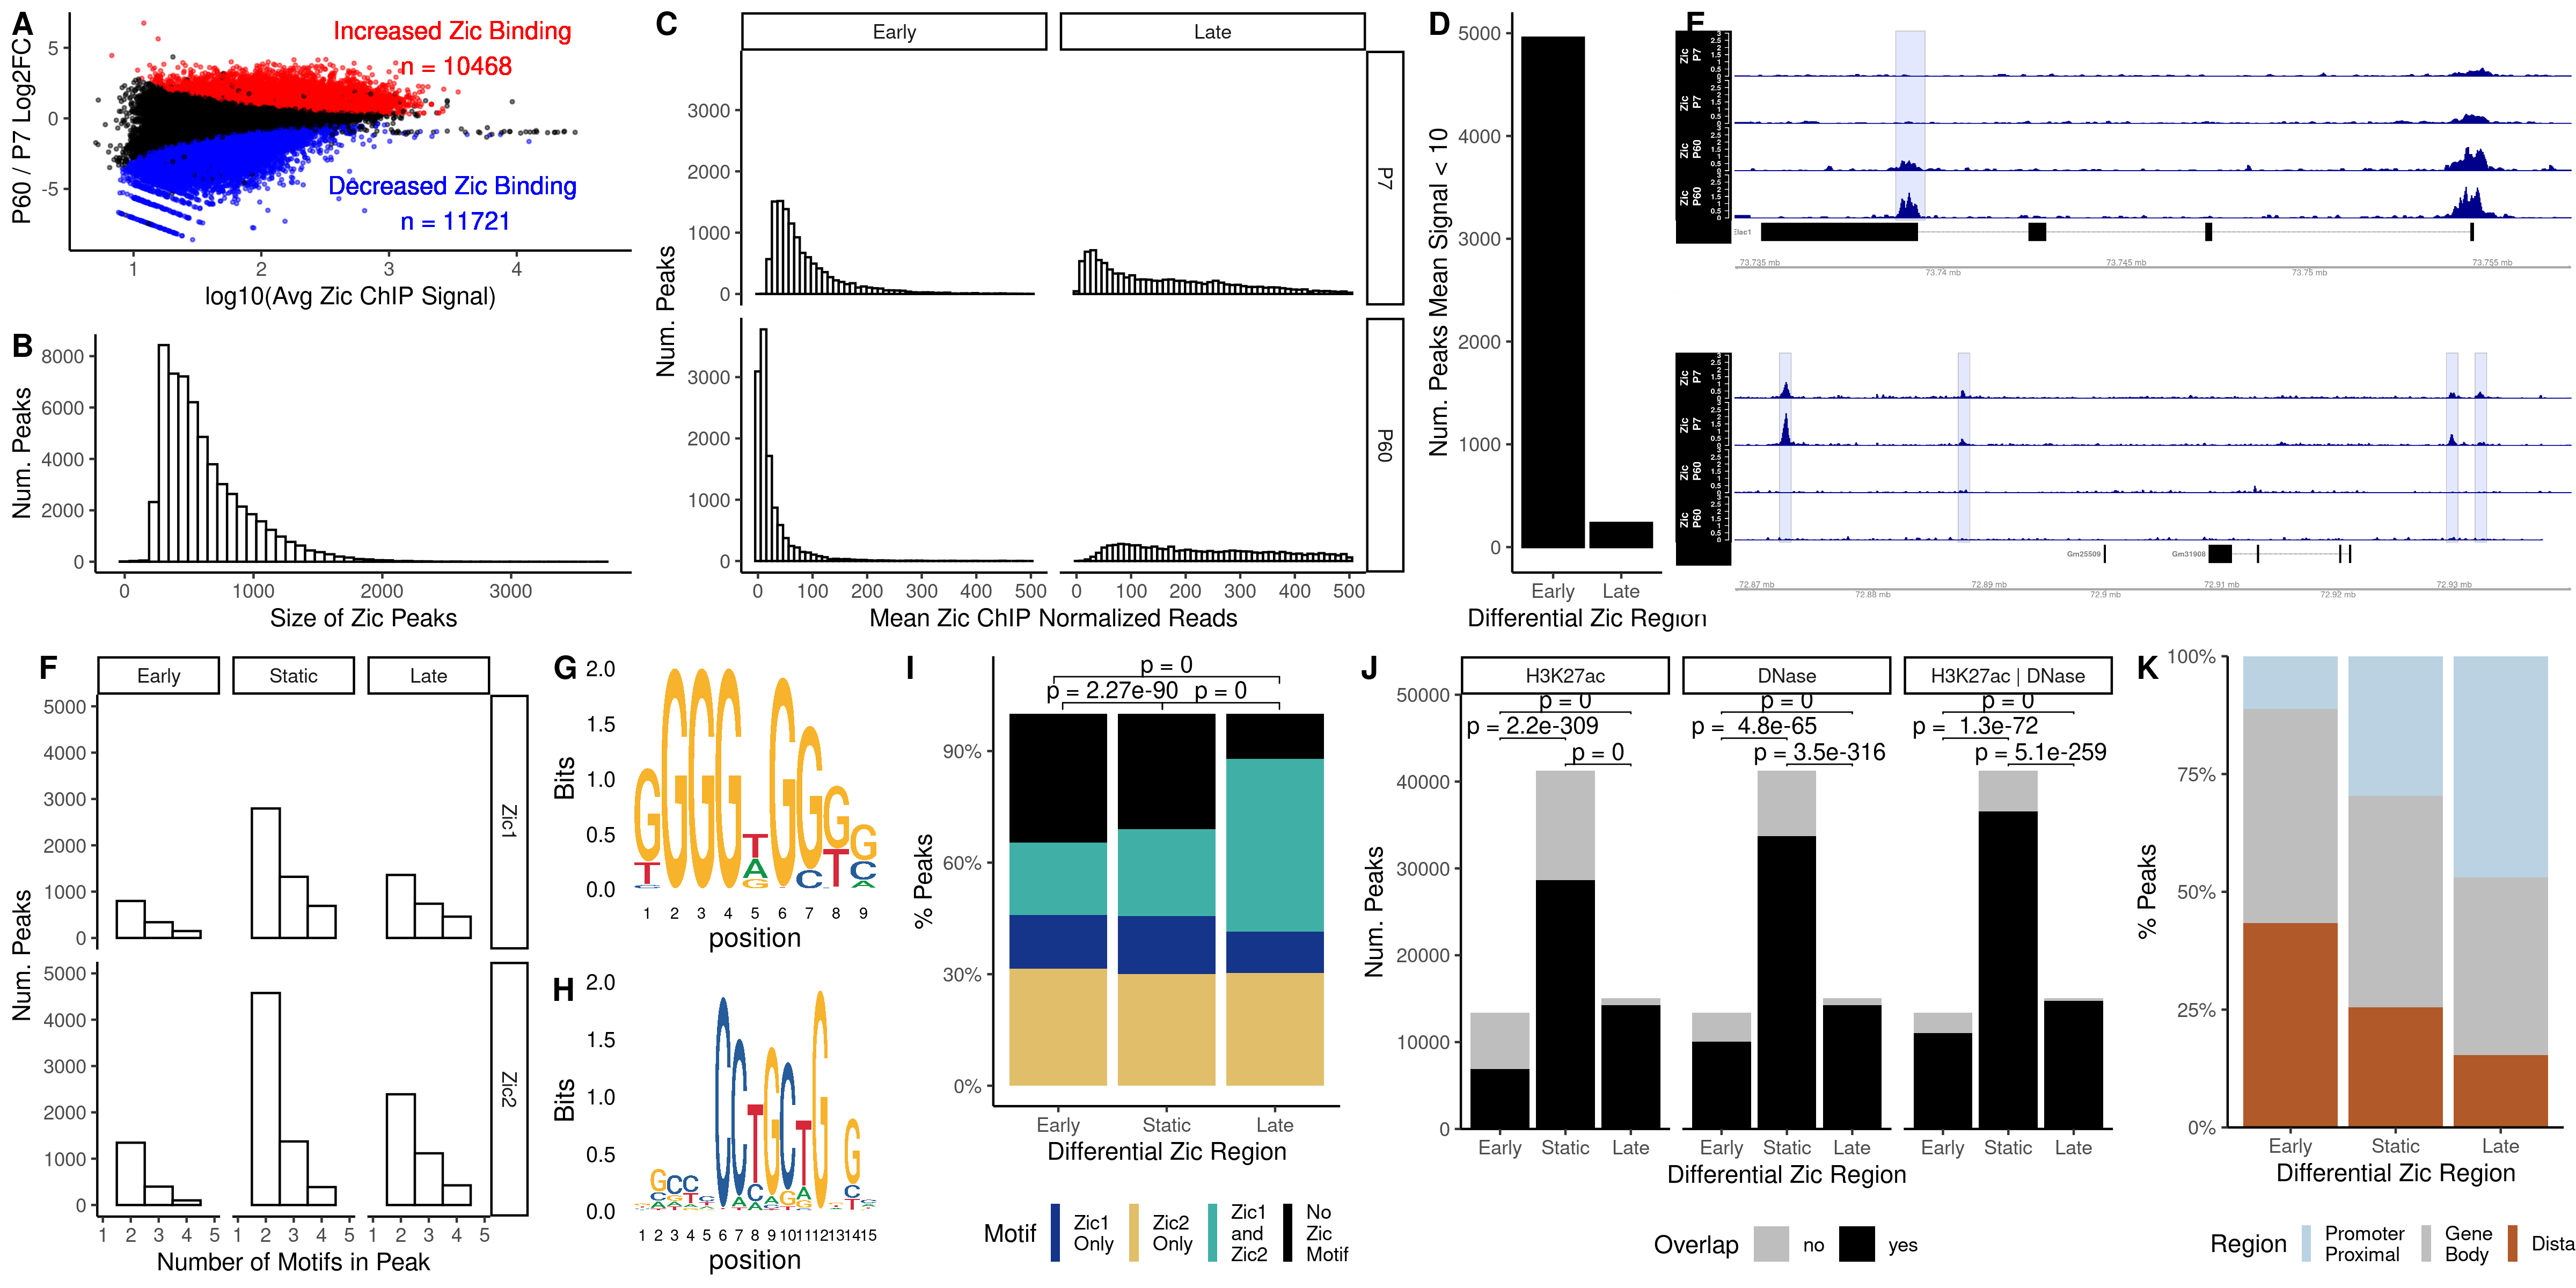
\includegraphics[width=.95\textwidth]{../figures/figure1.png}
\caption{ Zic1/2 Binding is dynamic across cerebellar development. A) MA plot comparing Zic ChIP binding at postnatal day 7 (P7) and postnatal day 60 (P60). B) Out of the thousands of peak that are differential between P7 and P60 only about ~400 were comletely lost or gained. C) Normalized expression of Zic1 and Zic2 show that thier respective genes are constitutivelt expressed during the development of the cerebellum. D) Zic binding highly overlaps wthh open chromatin (Dnase) and H3K27ac. E) Sites that overlap in chromatin accesibility tend to overlap with H3K27ac. F) Within these Zic binding sites, there Zic1 and Zic2 motifs can be found. G) The genmic loci of Zic ChIP peaks change from P7 and P60. }
\label{fig:ZicPeaks}
\end{figure*}


\section*{Results}

\subsection*{Zic binding shifts from enhancers to promoters throughout CGN maturation} 
We first sought out to characterize the differences in the location Zic ChIP binding in early versus late CGN development. Differential binding analysis of Zic1/2 ChIP peaks were performed Differential binding analysis between 56,941 merged Zic ChIP peaks at P7 and P60 showed  10,488 sites increasing in binding and 11,721 sites decreasing in binding (Figure\ref{fig:ZicPeaks}A). Interestingly, there were very few peaks that were novel but instead binding either increeased or decreased in binding intensity. There are l>400 peaks that are completely lost and fewer than 5 that are completely gained (Figure \ref{fig:ZicPeaks}B). Zic binding in early and late maturation did not differ in its preference to bind to active chromatin regions which was marked by DHS sites and H3K27ac binding (Figure \ref{fig:ZicPeaks}D). Majority of the peaks that overlap in DNase also overlaps with H3K27ac (Figure \ref{fig:ZicPeaks}E). Interestingly, one major difference between the binding profile of Zic between P7 and P60 is the where in the genome Zic is binding. There is a shift from Zic binding at distal enhancer regions at P7 and promoter regions at P60 (Figure \ref{ZicPeaks}G). 

To determine whether the Zic1/2 ChIP was capturing differences in Zic1 and Zic2 binding over development, we examined the motif occurrence of Zic1 and Zic2 in each peak. We find that most peaks either have the Zic1, Zic2, or both Zic1 and Zic2 motifs within each peak (Figure \ref{fig:ZicPeaks}F) which proportionally do not change between P7 and P60. 



\subsection*{Distinct TFs enriched in Early and Late Zic Binding sites}

\begin{figure*}[!ht]
\centering
\includegraphics[width=.95\textwidth]{Figures/figure2_alt.png}
\caption{A) Schematic for finding disitnct TF enrichment between two peaksets. Distinct TFs enriched between early and late regulatory modes. A ranked hyper-geometric overlap test was performed to identify the TFs distinctly enriched in each set. Then the proteins were mapped to their respective gene expression. C) Distinctly enriched B) motifs and C) ChIP overlap between early and late zic binding. D) E) Log fold change of genes mapped to distinct TFs.  }
\label{fig:DistinctTFs}
\end{figure*}

We next asked what is causing differential tar getting of Zic binding between P7 and P60. We hypothesized that a other co-factor maybe driving its targeting. A multi-pronged approach was used to get the TFs whose binding is enriched using BART \cite{Zhenjiawang2018BART:Profiles, Ma2021BARTweb:Analysis} as well as TFs whose motifs are enriched at these loci using Homer \cite{}. This allows interrogate direct and indirect binding by examining motif and ChIP overlap enrichment respectively. Then a Rank-Rank Hyper-geometric overlap test was used to compare the TF enrichment of two peak sets resulting in a list of TFs that are distinctly enriched in either set. To further determine putative co-factors of Zic, each predicted TF whose motifs or ChIP profiles were distinctly enriched was mapped to its corresponding gene then filtered for being developmentally expressed  (Figure \ref{fig:DistinctTFs}A). This way only TFs who are distinctly enriched in either peak set and also differentially expressed during development was considered a putative TFs driving differential targeting of Zic. This workflow revealed a set of distinct TFs enriched at Zic binding sites in early and late development (Figure \ref{fig:DistinctTFs}B-C).

\subsubsection*{Many more TFs shown to bind in-vivo than predicted motifs} 
Even though there is great overlap in the set of TFs in both the BART and HOMER databases (Figure \ref{fig:HomerBart} A), there are more predicted TFs that bind in-vivo than by motif enrichment (Figure \ref{fig:HomerBart}). Moreover, many of the predicted TFs with enriched motifs are not enriched by ChIP profiles. While some of this may be attributed to the different sets of TFs used in the Homer and Bart tools (Figure \ref{fig:HomerBart}A), it still suggests suggests that there are many TFs that are indirectly bound at these Zic bound chromatin loops. Additionally, many of these enriched TFs are not concordantly transcriptionally enriched at the time point in which their motif or ChIP binding is enriched. For discordant TFs that are transcriptionally enriched early but sequence is enriched in late Zic peaks, we speculate that these are recruiters or placeholders for late Zic binding. Similarly, TFs that are transcriptionally enriched late but sequence is enriched in early Zic peaks, we think these are hand-off factors of early Zic binding.

\subsection*{Workflow captures previously identified TFs known to work with Zic in early neurogenesis}
Motifs that were enriched early and expressed early include factors involved in cell proliferation via FGF and Notch signalling cascades (Figure \ref{fig:DistinctTFs}D,E). Enriched TFs in early Zic sites in the cerebellum involved in these pathways include  Maz and Tfap4 upstream of Wnt signalling \cite{Martinez2020TheDevelopment, Song2018TranscriptionCarcinoma}, TCF proteins as a part of the $\beta$-catenine pathways, and RFX proteins upstream of FGF activation \cite{Hsu2010RegulationRFX1}. FGF and Notch signalling have been proposed to work concurrently to lead to neurogenesis \cite{Voelkel2014FGFHierarchy} whereas Wnt signalling plays a context dependent role in neurogenesis \cite{Lassiter2014SignalingDelamination}. Zic1/2/3 is known to block Wnt-$\beta$-catenin signalling binding directly to TCF proteins of the $\beta$-catenin complex \cite{Ge2020Zic1Transition, Fujimi2012XenopusPathway, Murgan2015AtypicalPrecursors, Pourebrahim2011TranscriptionSignaling, Aruga2018ZicDisease,Aruga2018Zic1,Lowenstein2021Olig3Development}. The linker protein H1.0 (H1f0) that is associated with proliferation and differentiation is also an enriched protein in early Zic binding \cite{DiLiegro2018H1.0Differentiation}. Downstream targets of Wnt and FGF signalling that drive cell proliferation and neurogenesis that are enriched include Atoh1, Ascl1, Stat3, and Neurog2 \cite{Dennis2019BHLHReprogramming}. Overall, Zic peaks at P7 were enriched for Homeobox and bHLH factors TF (Figure \ref{}). This is consistent with previous studies implicating Zic as a regulator of pro-neural bHlH factors in early proliferative stages neuronal differentiation \cite{Aruga2018ZicDisease}. Overall, Zic peaks at P7 were enriched for Homeobox and bHLH factors TF (Figure \ref{}). This is consistent with previous studies implicating Zic as a regulator of pro-neural bHlH factors in early proliferative stages neuronal differentiation \cite{Aruga2018ZicDisease}. 

% SMAD5 --> nodal signalling
Most notably, the TF is Atoh1 is greatly transcriptionally enriched at P7 (Figure \ref{fig:DistinctTFs}D). In the Cerebellum, the bHlH factor, Atoh1 has been shown to be expressed in the rhombic lip progenitor zone to regulate the expression of other TFs such as Pax6 and give rise to cerebellar granule neurons between the stages of E12.5 - P14 \cite{Aruga2018ZicDisease, Yeung2014WlsDevelopment, Wang2005Math1Cerebellum, Ben-Arie1997Math1Neurons}.To validate the predicted co-factors of Zic in early and late CGN development, we examined the overlap of binding profiles of available ChIP-seq data in the developing mouse cerebellum  (Figure \ref{fig:chip_overlap}. The overlap of CGN fate-determining TF Atoh1, chromatin remodelers Chd4 and Chd7 with developmental Zic ChIP-seq peaks was calculated. \ Comparing Atoh1 ChIP peaks to developmentally regulated Zic peaks reveal that ~55\%  Atoh1 ChIP peaks does in fact overlap with Zic peaks (Figure \ref{fig:chip_overlap}A). Atoh1 ChIP overlaps at P7 enriched peaks at a greater percentage than peaks that are static and peaks enriched at P60 (p-value < 0.05) (Figure \ref{fig:ZicPeak}E). These results validate that this workflow that integrates gene expression and sequence underlying ChIP peaks to predict TFs that are enriched in a developmental context.


\subsubsection*{Chromatin repressive complexes are early collaborators of Zic}
There is strong signature of chromatin remodeling factors whose ChIP binding profiles strongly overlap early Zic binding. TFs that are members or interact with of cohesin complex  (CTCF, Rad21, Stag1, Smc3), Polycomb  complex (BMI1, Phc1, Pcgf2, Arid3a ), HP1 complex (Cbx5, Cbx3), Nurd Complex (Trim28, Mbd3), REST complex and BAF complex ( Top2b, Smarcad1) are distinctly enriched in early Zic binding (Figure\ref{fig:DistinctTFs}E). 

Members of Cohesin are enriched at the early Zic sites including CTCF, Rad21, and Smc3. Studies have shown that the 3D architecture of the genome is dynamic between early development and cell fate commitment. While TAD boundaries are relatively stable, local chromatin can undergo massive reorganization as cells respond to signalling or developmental cues which is correlated with changes in gene expression\cite{Zheng2019TheDifferentiaition, Bonev2016OrganizationGenome}. 

For instance, the polycomb complex is linked with maintaining the repression of pluripotency genes \cite{Riising2014GeneWide}. BMI1 and Pcgf2 the major ring  and core components of PRC1 whose role is to maintain repression of genes \cite{Aranda2015RegulationProteins}. Interestingly, Phc1 whose binding is enriched in early Zic sites, has recently been shown to activate  Nanog in a PRC1-independent manner and repress developmental genes in a PRC1-dependent manner \cite{Chen2021Phc1Locus}. 
% Arid3a 

Collaborators of the BAF complex to drive and maintain proliferation were found enriched at early Zic sites. Top2b, a collaborator of BAF to recruit pluripotency pioneer factors including Oct4 and Nanog, was enirched at early Zic sites. Similarly,  Smarcad1, a subunit of BAF that has been shown to be involved in Histone H3/4 turnover \cite{Markert2021Smarcad1Activity}, was  enriched at early Zic sites. BAFs have a varying roles in different stages of development and in response to cell signalling. The nBAF complex has roles in dendritic development and neuronal maturation. \cite{Alfert2019TheDisease}. Interestingly, the core component of esBAF is required to induce accessibility at targets of pluripotency genes thus preventing polycomb repression \cite{Ho2011EsBAFFunction}.  Additionally, TF enrichment of Hic1, a transcriptional repressor of Atoh1 \cite{Briggs2008CooperationMedulloblastoma },interacts with SWI/SNF/BAF chromatin remodeling complex via the Arid1 sub-units and NurD complex via MTA1 \cite{VanRechem2009HIC1ARID1A/BAF250A, VanRechem2010DifferentialCells}, and competitively recruits TCF4 away from $\beta$-catenin \cite{Valenta2006HIC1bodies} to end cell proliferation. The TF REST, which is enriched in early Zic sequences, works to recruit epigenetic silencing machinery like HP1, and Mecp2 to silence neuronal genes \cite{Ballas2005TheGenes}. Additionally, in the absence of REST, Pax6-containing BAF complex is known to activate genes in neurogenesis \cite{Ninkovic2013TheNetwork, Tuoc2013ChromatinThickness}. 

%A recent study has shown that activity induced phosphorylation of BAF leads to enhnacer and promoter looping and decrease of NuRD repressor complex \cite{Kim2021NeuronalActivation}



Trim28 can recruit repressive chromatin complexes including NuRD and HP1 \cite{Sripathy2006TheRepression}. Zic2 has been shown to interact with the Chd4-Mdb3-containing NuRD complex to maintain pluripotency in cells\cite{Luo2015Zic2Specification}. Early enriched factors, CBX3 and CBX5 are components of HP-1 and function as readers of H3K9me2/3 \cite{vanWijnen2021BiologicalDevelopment}. Readers (CBX3, CBX5) and writers of histone methylation  (Ehmt2,Kdm4b, Mecp2),  removers of histone acetylation (Hdac2), and the transcriptional repressor Tgif2  are distinctly enriched at early Zic sites sites. Taken together, this suggest that Zic binding overlaps with targets of with different chromatin modifiers involved in chromatin repression to main cell proliferation signals in early postnatal development. 

% XBP1, ZSCANN22 

\subsection*{Modes of Late Zic binding}
Unlike the factors enriched early that have a overwhelming presence in chromatin remodeling and repression, the factors enriched late can be split into two groups: 1) Factors that are transcriptionally enriched early that are involved in transcriptional regulation 2) Factors that are transcriptionally enriched late that is either 2) involved in rentinoic acid signalling or 3)  show signatures of activity regulated gene expression. 

\subsubsection*{Putative recruiters of Zic include proliferation markers and repressive complexes}
The late sites are enriched for TF binding of factors that are transcriptionally enriched early are potential recruiters or placeholders for late Zic binding (Figure \ref{fig:DistinctTFs}D). These factors including EBF1, ZNF768, Mybl2, and E2F7 are associated with cell proliferation. Both EBF1 and ZNF768 both predicted regulate transcription via RNA POLII. ZNF768 has been further shown to regulate genes involved in cell proliferation \cite{Villot2021Znf768Fingers}. Mybl2 is a cell cycle dependent gene \cite{Liu1996CellElement}. Overexpression of E2F7 promotes cell proliferation and is an activator of EZhH, the core component of PRC2 \cite{Yang2020E2F7EZH2Progression}.  Being that these markers are transcriptionally enriched early, we think that the factors that drive proliferation was later recruited by Zic1/2 to transition the progenitor pools into mature post-mitotic cells.
%tcf3 not mentioned 

Repressive signatures are found in sites that recruit Zic. DNMT3B is a methyltransferase that deposits de novo and maintain DNA methylation  during embryonic stages of development. HP1 stabilizes its binding to H3K9me3 and EZH2 recruits its binding the H3K27me3 \cite{Gagliardi2018Dnmt3bDisease}. UBTF has recently been proposed to serve as a integral structual support of TAF1 binding, a RNA POL pre-initiation complex \cite{Tremblay2022RibosomalSyndrome}. Phf6 is needed for neuronal growth and interacts with Ubtf, Hdac, and NuRD. Phf6 KO suggest that it regulates components of the BAF complex \cite{Fliedner2020LossCells}. CBX2 a H3K27me3 reader and PCGF6 are both components of PRC1\cite{Aranda2015RegulationProteins}. Arid1a is a core BAF complex sub unit important throughout development  \cite{Alfert2019TheDisease}. Erf is a transcriptional repressor \cite{Sgouras1995ERFStimulation}. Sin3a forms a  complex with HDACs. The Sin3a-HDAC complex co-occupies Nanog binding which is required for pluripotency \cite{Saunders2017ThePluripotency}. Interestingly, ChIP binding of Atoh1 is enriched in Late Zic sites suggesting that Atoh1 may bind indirectly at some sites to later recruit Zic. 

Signatures of Wnt and Notch signalling enriched in late sites (Notch1, Hey1, MycN, Med12). Notch signalling drives proliferation in Granule Neurons and when turned off, differentiation occurs \cite{Adachi2021NotchProgenitors}. Hey1 is activated downstream of Notch signalling \cite{Nandagopal2018DynamicPathway, Yoon2005NotchMutants}. Mycn activates Notch signalling via transcriptional activation of Hes1 \cite{Tong2019Mycn-MeidatedApoptosis}.
Med12 is an important suunit of the mediator complex and is recruited to Wt/$\beta$-catenine target genes to activate transcription \cite{Kim2006MeidatorSignaling}

% ^ This is again just a list of facts--try to identify the key ideas or groups here, and bring it back to a model of how these factors may be interacting with Zic binding

\subsubsection*{Late collaborators of Zic and  Retinoic acid signalling}
Retinoic acid signalling is thought to be a key switch from neuronal proliferation to neuronal differentiation \cite{Janesick2015RertinoicDifferentiation}. The RAR complex repressed REST which then allows for microRNA mediated depletion of npBAF and up-regulation in nBAF which is important in post-mitotic neurodevelopment \cite{Alfert2019TheDisease}. Here we show that rora and rorc are distinctly enriched at late Zic sites during stages of cerebellar maturation (Figure\ref{fig:DistinctTFs}D). Other TFs that are markers of differentiation include, Klf4, it induces expression of p21 which suppresses cell proliferation \cite{Zhang2000ThePromoter}. Pol3gl is a subunit in RNA Pol III which functions to transcribe small non-coding RNAs, has been implicated in cerebellar development, and downstream of Nanog, a pluripotency maintainer\cite{Wang2020FunctionsDevelopment}.

Hif1a which is induced after hypoxic stress can up-regulate miR-125 which works through several mechanisms to activate Wnt/$\beta$-catenin and Notch signalling \cite{Jiang2020HIF-1-regulatedSignaling}. Xbp1 can form a complex with Hif1a to regulate expression of its downstream targets \cite{Chen2018Xbp1Pathway}. However, Wnt/$\beta$-catenin signalling can destabilize the Xbp1-Hifla complex in a negative feedback loop \cite{Xia2019HypoxicSurvival}.
- Controls onset of neuronal proliferation

Still at late sites, Cbx7 binding,  a subunit of PRC1 and is associated with transcriptional repression of lineages specific genes \cite{Aranda2015RegulationProteins} is enriched. 


\subsubsection*{Activity Regulated Genes collaborate with Zic in later stages of cerebellar maturation}
Canonical activity regulated genes have binding sites enriched in late Zic peaks including Fosl2, Fos, Jun, Egr1, Mef2a, and Mef2d. Although Nfil3 has been mostly researched in the context of immunology, it has been shown to be up regulated in the hippocampus in response to fear conditioning \cite{Mizuno2020Long-lastingConditioning}.

The Ap-1 complex is a heteroodimer comprised of Fos and Jun TF members that can also dimerize with factors such as Egr1 and ATF factors \cite{Raivich2006RoleBrain}. These are common response factors to stress in the cerebellum \cite{Nakamura2015ExpressionActivity, Coffey2000DualNeurons}. Increases in c-jun expression are seen after neuronal injury \cite{Liu2000TranstentorialMice}, memory and learning in the cerebellum, and required for axonal regeneration \cite{Raivich2004TheRegeneration, Raivich2006RoleBrain}. Previously, AP-1 was not seen in the cerebellum during early post-natal development \cite{Guerrini1997Glutamate-DependentDevelopment}. However, this data shows that members of the AP-1 complex are up-regulated in late postnatal cerebellum consistent with another study that shows downstream factors of AP-1 such as JNK and MEKs are up-regulated throughout late stages of CGN maturation \cite{Coffey2000DualNeurons}. These findings are consistent with idea that activity related genes (ARGs) are necessary for synaptic maturation\cite{West2011NeuronalFunction} and more specifically that Fos expression is required for activity induced chromatin accessibility of Fos binding targets\cite{Su2017NeuronalBrain} which is needed for sensory driven synapse elimiantion. 

Aff4 is a subunit of the Super Elongation Complex that is associated with paused RNA Pol II for rapid transcription. Aff4 targets Myc and factors involved in RNA Pol stabilization \cite{Luo2012TheControl}.

%ERG1 is NMDAr-depndednt\cite{Kim2018SynapseGenes}

\subsection*{Purkinje Cell Predicted TFs}
Although these data are derived from whole cerebellum, only a few predicted TFs have been strongly associated with the other cell types in the cerebellum. Olig2, Ptf1a, NueroG2, Ascl1 are expressed highly and distinctly in the ventricular zone in the embryonic phase in cerebellum which gives rise to Purkinje cell lineages \cite{Lowenstein2021Olig3Development}. RORa is expressed in mature postnatal Purkinje and RORa deficient mice show a significant reduction of Purkinje cells \cite{Jetten2006RetinoidrelatedDevelopment}. The TFs in the TEA Domain family, including TEAD4, is an important regulator downstream in the Hippo signalling pathway. They work as DNA binding guides to core kinases in the Hippo signalling pathway resulting in cell proliferation and differentiation  \cite{Lavado2018TheNumber, Jin2020TheDiseases}. They have been shown to regulate signalling in Purkinje cells to maintain proper cellular morphology \cite{Jin2020TheDiseases}. For these reasons, we conclude that these TFs are not working with Zic to drive maturation of CGNs but TFs working in the Purkinje cells.

%You can organize this more along the lines of 'while the cerebellum is mostly homogenous, there are other cell types, including PCs. These TFs which emerged from our analysis have previously been shown to act in PCs in this way. Therefore, although our method was sensitive enough to detect this signature from a minority cell population, we attribute this signal to contamination from the PCs.

%ROrc, rora, teadr4 expressed in GC!

\subsection*{Workflow captures previously identified TFs known to work with Zic in early neurogenesis}

%Some of the predicted TFs enriched at P7 Zic sites have been described up and downstream of the Zics in several pathways in embryonic development (Ets1, Pax6, Meis1, Tbr1, BMyb, Oct6, Srebf1, Brn2, Asc11) \cite{Aruga2018ZicDisease, Fink2006DevelopmentLip, Shepard2005ASusceptibility, Buecker2014ReorganizationPluripotency, Toledo2020Srebf1Neurogenesis, Urban2015ACells, Sankar2016GeneZic1}. TCF proteins have been demonstrated to bind with Zic2 to repress  Wnt/$\beta$-catenin signalling \cite{Aruga2018Zic1, Lowenstein2021Olig3Development}. The Tgif factors and Bcl11a have implicated in cerebellar malformations such as holoprosencephaly human and mouse \cite{Aruga2018ZicDisease, Shimbo2017HaploinsufficiencySyndrome}. Overall, Zic peaks at P7 were enriched for Homeobox and bHLH factors TF (Figure \ref{fig:ZicPeak}C). This is consistent with previous studies implicating Zic as a regulator of pro-neural bHlH factors in early proliferative stages neuronal differentiation \cite{Aruga2018ZicDisease}. 

To validate the predicted co-factors of Zic in early and late CGN development, we examined the overlap of binding profiles of available ChIP-seq data in the developing mouse cerebellum  (Figure \ref{fig:chip_overlap}. The overlap of CGN fate-determining TF Atoh1, chromatin remodelers Chd4 and Chd7 with developmental Zic ChIP-seq peaks was calculated. Most notably, the TF is Atoh1 is greatly transcriptionally enriched at P7 (Figure \ref{fig:DistinctTFs}D). In the Cerebellum, the bHlH factor, Atoh1 has been shown to be expressed in the rhombic lip progenitor zone to regulate the expression of other TFs such as Pax6 and give rise to cerebellar granule neurons between the stages of E12.5 - P14 \cite{Aruga2018ZicDisease, Yeung2014WlsDevelopment, Wang2005Math1Cerebellum, Ben-Arie1997Math1Neurons}. Comparing Atoh1 ChIP peaks to developmentally regulated Zic peaks reveal that ~55\%  Atoh1 ChIP peaks does in fact overlap with Zic peaks (Figure \ref{fig:chip_overlap}A). Atoh1 ChIP overlaps at P7 enriched peaks at a greater percentage than peaks that are static and peaks enriched at P60 (p-value < 0.05) (Figure \ref{fig:ZicPeak}E). These results validate that this workflow that integrates gene expression and sequence underlying ChIP peaks to predict TFs that are enriched in a developmental context.

% Zic1 directly represses Atoh1 \cite{Ebert2--3Zic1Autoregulation}




\subsection*{Mapping Peaks to Genes via chromatin loops to determine enhancers mediated by Zic}

\begin{figure*}[!ht]
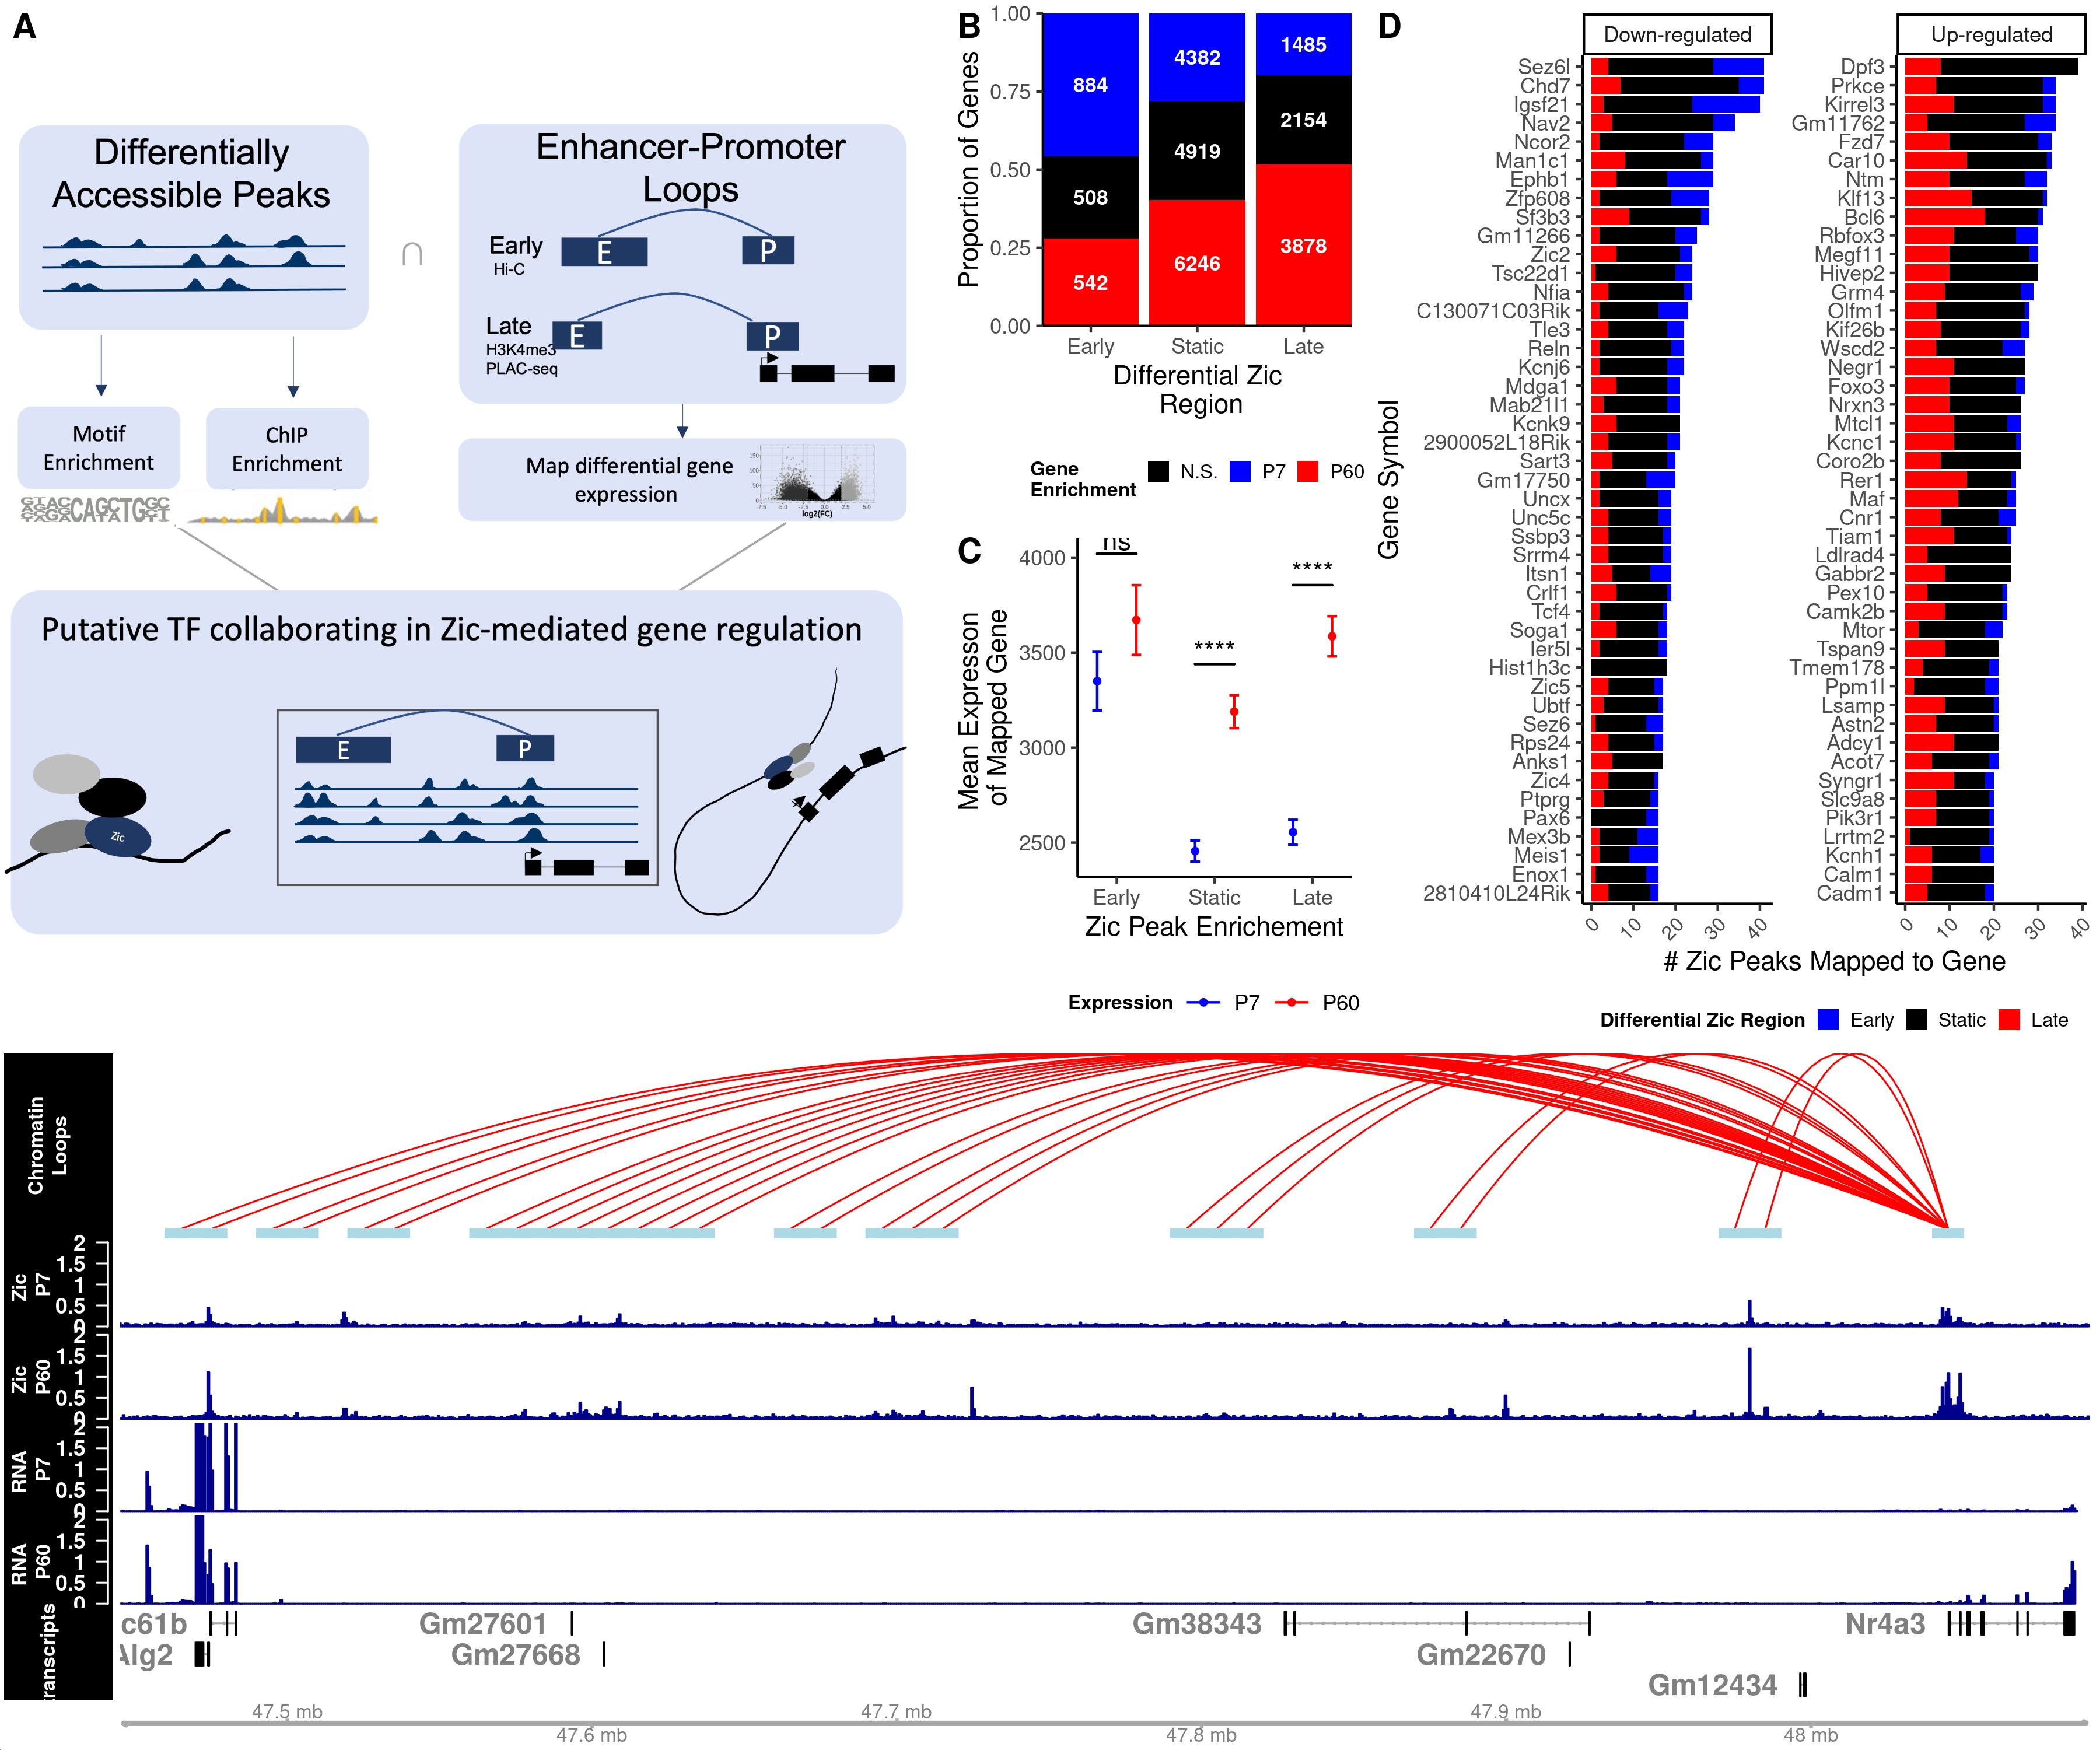
\includegraphics[width=.95\textwidth]{Figures/figure3.png}
\caption{Zic peaks were mapped to genes via H3K4me3 mediated chromatin loops. A) Overall number of genes mapped to Zic peaks that are enriched at P7, P60, and Statically bound. B) Mean expression of genes at P7 and P60 mapped to P7 and P60 enriched Zic peaks. C) Top 50 number of Zic peaks mapped to genes that are differentially expressed between P7 and P60. D) Example tracks of H4Kme3 loops, Zic, DHS, H3k27ac, and Gene expression at P7 and P60}
\label{fig:PeakMapping}
\end{figure*}

Enhancer promoter loops captured from young and adult cerebellum allow us to map Zic peaks to genes to determine Zic's regulatory modes. H3K4me3 chromatin loops in adult mice cerebellum \cite{Yamada2019SensoryLearning} and Hi-C chromatin loops in young mice \cite{Goodman2020TheBrain}  were used as a proxy of promoter-enhancer looping in the mouse cerebellum  to map Zic bound enhancers to genes in the developing cerebellum. Peaks within the anchors of these predicted chromatin were mapped to genes (Figure \ref{fig:PeakMapping}A Figure \ref{fig:MappingStats}). With this method, long range peaks can be more confidently mapped to distal genes. These mapped Zic peaks were interrogated for motif enrichment and TF binding enrichment to further investigate the regulatory modes of Zic and its binding partners. 

%Direct target of genes of Zic, there is not a solely activating or repression 

\subsubsection*{Many Zic peaks map to a single gene}
Surprisingly, this revealed that there are many Zic peaks that map to a single gene (Figure \ref{fig:nPeakstoGenes}D, \ref{fig:PeakMapping}C). We next asked, if the number of Zic binding events was a proxy of regulatory activity by asking if expression or fold change in expression was a function of the number of Zic peaks. There is no correlation between the number of Zic peaks and distribution of the mapped gene LFC, average expression or degree of fold change (Figure \ref{fig:nPeakstoGenes}B-D). Thus, Zic binding does not have an additive effect on gene regulation. 

%\subsubsection*{Differences in the Plac-seq and Hi-C data}
%% add sesction here about the young v old loops 
%- describe differnces in data 
%- and why we think its not changing


\subsubsection*{Zic Peaks can be classified as activators or repressors}
Zic peaks were mapped to genes that were up-regulated and down-regulated consistent with findings of Zic may have multiple regulatory modes \cite{Ishiguro2018LinkExpression, Himeda2013Pax3Enhancer}. The mean expression of genes mapped to Static and P60 Zic peaks significantly increases between P7 and P60 (Figure \ref{fig:PeakMapping}B) suggesting that the P60 and static Zic peaks promote transcription. However, there is a many-to-one mapping of Zic peaks to genes and the regulation of these Zic peaks are not always congruent the regulation of the mapped gene (Figure \ref{fig:PeakMapping}D). 




%\subsection*{Zic plays an important role temporally}
%There were little to none distinctly enriched TFs in the activating v repressive sets (Figure %\ref{fig:ActvRep}) but in the early and late sets (Figure \ref{fig:DistinctTFs}.
%- dont think changes in Zic drives activation and repression
%- Zic is an activator because Zic overlaps with H3K27ac
%- correlation between zic binding regulation and gene regulation
%- however there is no difference in TFs between early zic binding and late zic binding
%- when zic is recruited to enhancers of Grin2c we see increase in gene expression of Grin2c %\cite{Frank2015RegulationCerebellum}
%
%%This suggest that rather than Zics having a direct role in gene activation or repression, they %are regulatory roles are more upstream to transcription. 
%
%- Zics have a non-linear relationship with targets
%- JUSTIFY COPARING TO RANDOM GENOMIC SEQUENCES
%
%To test, this we looked at the TFs enriched in the early and late Zic peaks that were mapped to %genes under the assumption that these peaks are of high confidence and involved minimally in the %epigenomic landscape of the developing cerebellum. Out of 205 enriched motifs, 20 are distinctly %enriched in the early peak set, and 27 and distinctly enriched in the late peaks set (Figure %\ref{fig:DistinctTFs} B,D). Out of the 326 TF whose ChIP binding were enriched in the early and %late peak sets, 42 were distinctly enriched early, and 22 were distinctly enriched late (Figure %\ref{fig:DistinctTFs} C,E).  
https://www.overleaf.com/project/61f2d442e6849f426be14e45

\begin{figure*}[!ht]
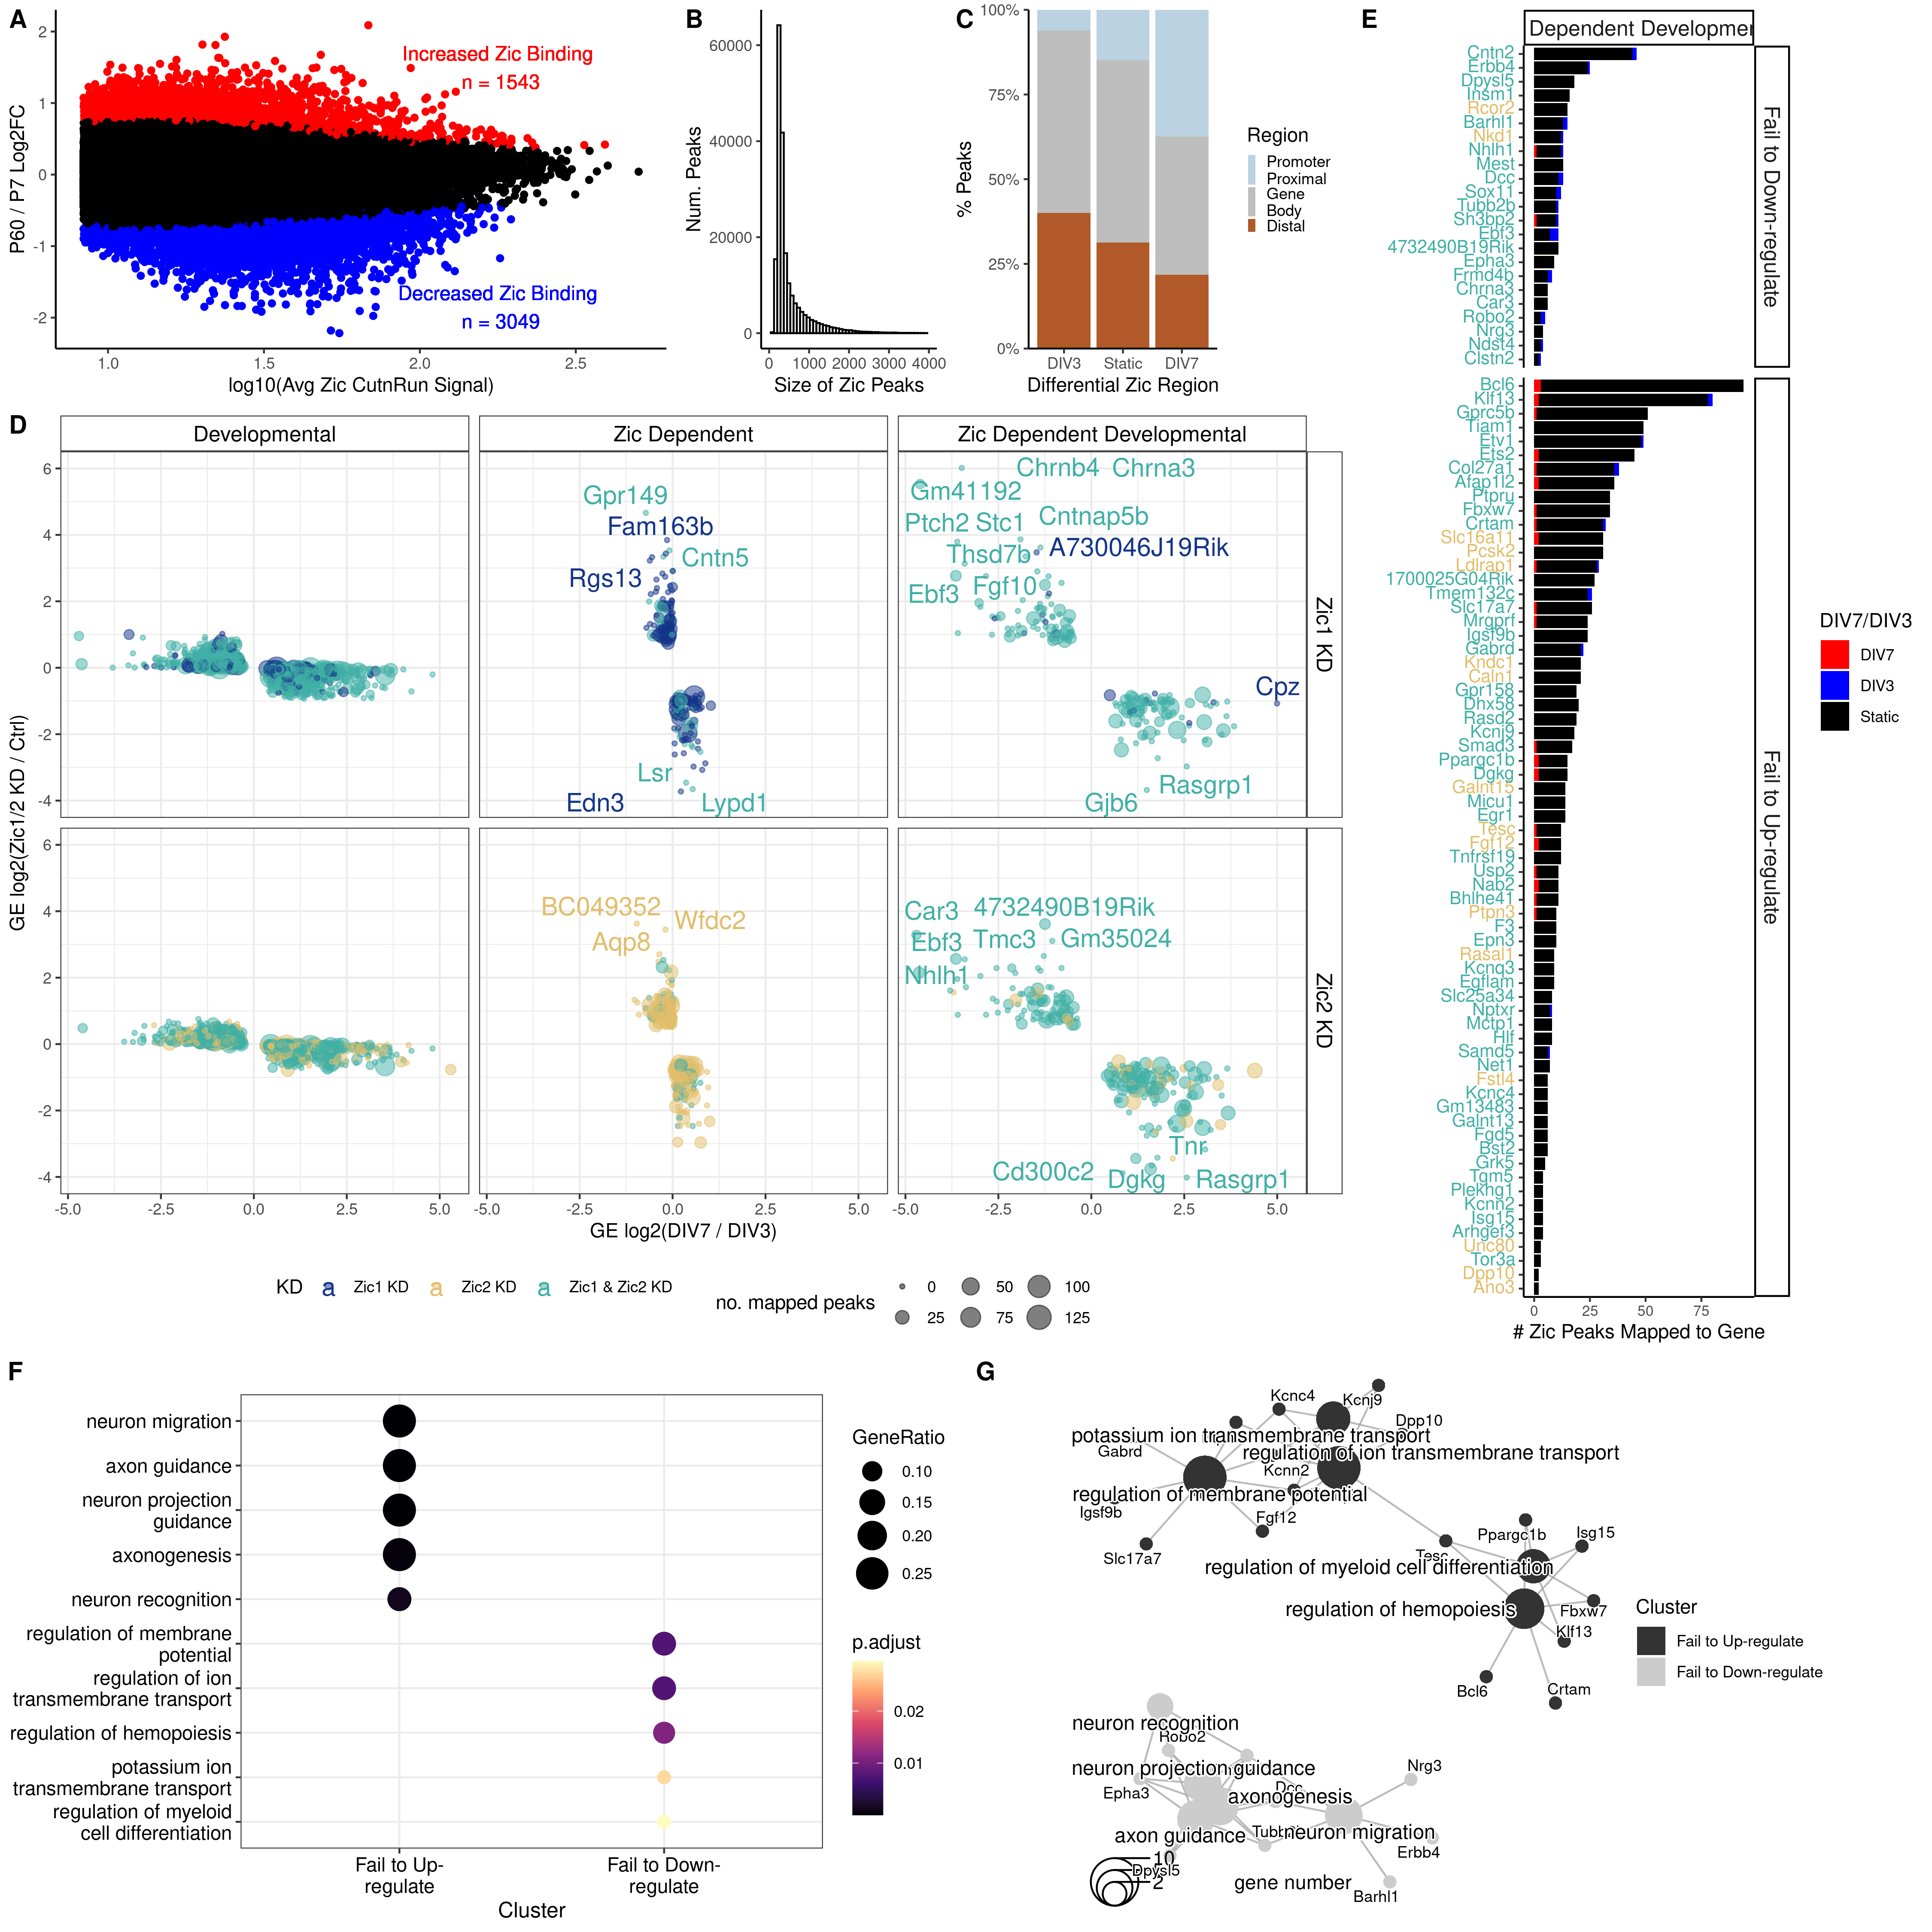
\includegraphics[width=.95\textwidth]{Figures/figure4.png}
\caption{}
\label{fig:ZicKD}
\end{figure*}

\section*{Peak mapping reveals Zic1/2 dependent developmental targets}
Granule cells were cultured and assayed at 3 days and 7 days in vitro to model CGN development. RRHO of the differential genes under WT conditions and in Zic1 and Zic2 KD was performed to assess the discordantly regulated genes. The discordant genes fell into three categories 1) Developmental: genes that did not change in either the Zic1 or Zic2 KD that were developmentally regulated in WT conditions(n=1582), 2) Zic Dependent (ZD): genes that did change in either the Zic1 or Zic2 KD that were not developmentally regulated (n=455), and 3) Zic Dependent Developmental (ZDD): genes that were dis-regulated by the Zic1 or Zic2 KD and are developmentally regulated (n=329) (Figure \ref{fig:ZicKD}A). Overall these genes showed signatures for neuronal markers that are important in development and synaptic refinement including axonogenesis, extracellular organization, and cell adhesion (Figure \ref{fig:ZicKD}B). 

Zic1/2 cut&run data was generated at DIV3 and DIV7 to determine whether Zic was binding at the enhancers or promoters of these genes. A select group of developmental genes (n = 62) and ZDD genes (n = 37) had Zic binding in regulatory regions of these genes. Peaks mapped to these genes were mostly statically bound. 



\section*{Discussion}

We sought out to determine the modes of Zic binding in the developing cerebellum by interrogating the sequence that underlies Zic peaks in early and late maturation. We implemented an integrative approach to enhance our understanding of Zic1/2 regulation on a molecular level. Although there were no differences between Zic peaks mapped to gene activation and Zic peaks mapped to gene repression, there was a clear difference between early and late Zic binding. While early Zic sites showed signatures of repressive chromatin remodeling complexes, the late Zic sites showed a novel set of activity regulated genes that are important in late neuronal maturation and synaptic refinement. 

% tgif2 is implcatedin holoproscencephalu


Many studies have implicated Zic in the maintenance of neuronal cell proliferation \cite{Lim2007Zic3Cells, Janesick2013ErfNeurogensis, Aruga2002Zic1Differentiation, Ebert2003Zic1Autoregulation}. Zic1 represses differentiation factors in order to increase cell number \cite{Aruga2002Zic1Differentiation}. RA signalling is thought to inhibit Zic expression \cite{Janesic2013ErfNeurogenisis} thus driving maturation.


Many of these temporally distinctly enriched factors whose functions involve cell proliferation are dysregulated in glioblastomas and other cancers. 

%glioma: mybl2, e2f7,hlf, zic1, dnmt3b, phf6, hey1
% EBF1: master regulator in B- and T-cels
% BACh2 - implicated in immune response, inflammation
% nr2f2 activated by ra signalling, implicated in immune response
% nfil3 - immune 
%hlf-tcf3 complex implicated in luekiemia




Factors that are likely to bot be CGN specific based off of the \href{https://apps.kaessmannlab.org/sc-cerebellum-transcriptome/}{sc transcriptome atlas} \cite{} are Olig2, Onecut2, Sox10, Nfil3, and Erf showing higher expression in oligodendrocytes. Ebf1, Tfap2a, and Nr2f2 showing higher expression in Purkinje cells. Tfap2a is activated downstream of Pft1a, a purkinje cell lineage marker \cite{Jin2015Tfap2aRetinogenisis, Lowenstein2021Olig3Development}. Chrm2 with higher expression in interneurons. Also, Klf4 showed no expression in any cell type in the cerebellum after E14.5. 


\section*{Methods and Materials}
\subsection*{ChIP-seq and DHS Data Analysis}
ChIP-seq reads were aligned to Gencode mm10 v. xx genome using \textt{STAR} v. xx. ChIP Peaks were called using \texttt{MACS2} v. xx with the parameters (\textt{ --narrow --no-model --ext 147}).  \texttt{bedtools2} merge was used to make a consensus peak and removing the mm10 blacklisted regions \cite{} for differential analysis. The peak count matrix was generated by getting the number of reads from the consensus set using \texttt{RSubreads::featurecounts()} v. xx. These counts were analyzed for Differential expression between P7 and P60  (p-value $< 0.05$). 


\subsection*{Identifying Distinctly Enriched  TFs between peak sets}
Peaks were categorized in peak sets based on the differential enrichment of the peak between P7 and P60 and the differential expression of the gene it was mapped to. If a peak was enriched near a gene that was also enriched, it was added to the activator set. Otherwise, if a peak was enriched but its nearest gene was not enriched, it was added to the repressor set. A multi-pronged approach was used to predict TF binding, a pwm-based method (HOMER v. xx) \cite{} to assess the motifs enriched at those sites and an data driven in-vivo based method (BART v. xx) \cite{Zhenjiawang2018BART:Profiles, Ma2021BARTweb:Analysis} to assess which TFs ChIP binding is enrched at these sites. To determine distinctly enriched TFs between peak sets a Rank-Rank hypergeometric overlap test \cite{RRHO} was performed that compared the ranked p-value of each TF  to calculate significantly concordant and discordant TF enrichment. This resulted in a subset of the enriched TFs in each peakset to be distinctly enriched in comparison to another peak set.  Each predicted TF or TF-fusion was mapped to its corresponding gene. Those distinctly enriched TFs between two sets were then filtered for normalized expression > 100 and being developmentally regulated (FDR < 0.05)

\subsection*{ChIP overlap analysis}
bedtools intersect was used to get the Zic peaks at each time-point that intersects with an Atoh1 ChIP, CTCF, Rad21, Chd4 and ChD7 ChIP datasets. The percent of overlap was calculated by examining how many Zic ChIP peaks had at least 1bp overlap with ChIP peaks from other datasets. 


\subsection*{Mapping peaks to genes via Chromatin loops}
ChIP peaks were mapped to genes using adult cerebellum H3K4me3 (promoter-enhancer) predicted loops \cite{Yamada2019SensoryLearning} and young Hi-C predicted loops \cite{Goodman2019RegulationRemodeling}. ChIP peaks that were within the 10kb anchor bins of these loops were considered within the promoter-enhancer interactions. The anchors of these loops were were mapped to its nearest genes using ChIPSeekR v. xx \cite{}. For each loop, the anchor with the closest gene was deemed the promoter anchor and the other anchor was deemed the enhancer anchor. The gene mapped to the promoter anchor was assigned to the loop. For cases where both anchors overlapped with gene promoters, then both anchors were deemed promoter anchors and both genes were assigned to the loop. ChIP peaks were assigned to loop anchors by way of intersection using \texttt{bedtools intersect}. Subsequently, the peaks intersecting the anchors of a loop was mapped to the genes assigned to the loop. Thus, distal and intragenic peaks were mapped to genes in a biologically relevant way using 3D organizational data from the same tissue type. Using this mapping, relationships between peaks and genes could be confidently assessed.  



\subsection*{Data Availability}
This the Zic ChIP and RNA-seq is as adapted from Frank et. al. 2015 \cite{Frank2015RegulationCerebellum} where the publicly available RNA-seq and ChIP-seq  data can be found here \href{https://www.ncbi.nlm.nih.gov/geo/query/acc.cgi?acc=GSE60731}{GEO:GSE60731}. Adult Plac-seq data is adapted from Yamada et. al. 2019 \cite{Yamada2019SensoryLearning} and publicly available here \href{https://www.ncbi.nlm.nih.gov/geo/query/acc.cgi?acc=GSE127995}{GEO:GSE127995}. Young Hi-C data is adapted from Goodman et al. 2019 \cite{Goodman2020TheBrain} and publicly available here:\href{https://www.ncbi.nlm.nih.gov/geo/query/acc.cgi?acc=GSE138822}{GSE138822}

\subsection*{Code Availability}
Scripts used for this analysis can be found in this GitHub repository: \href{https://github.com/MelyssaMinto/zic_analysis}{https://github.com/MelyssaMinto/zic_analysis}

\section*{Acknowledgments}



\bibliography{references}

\clearpage


\beginsupplement
\section*{Supplementary Material}

\begin{figure*}[ht]
\centering
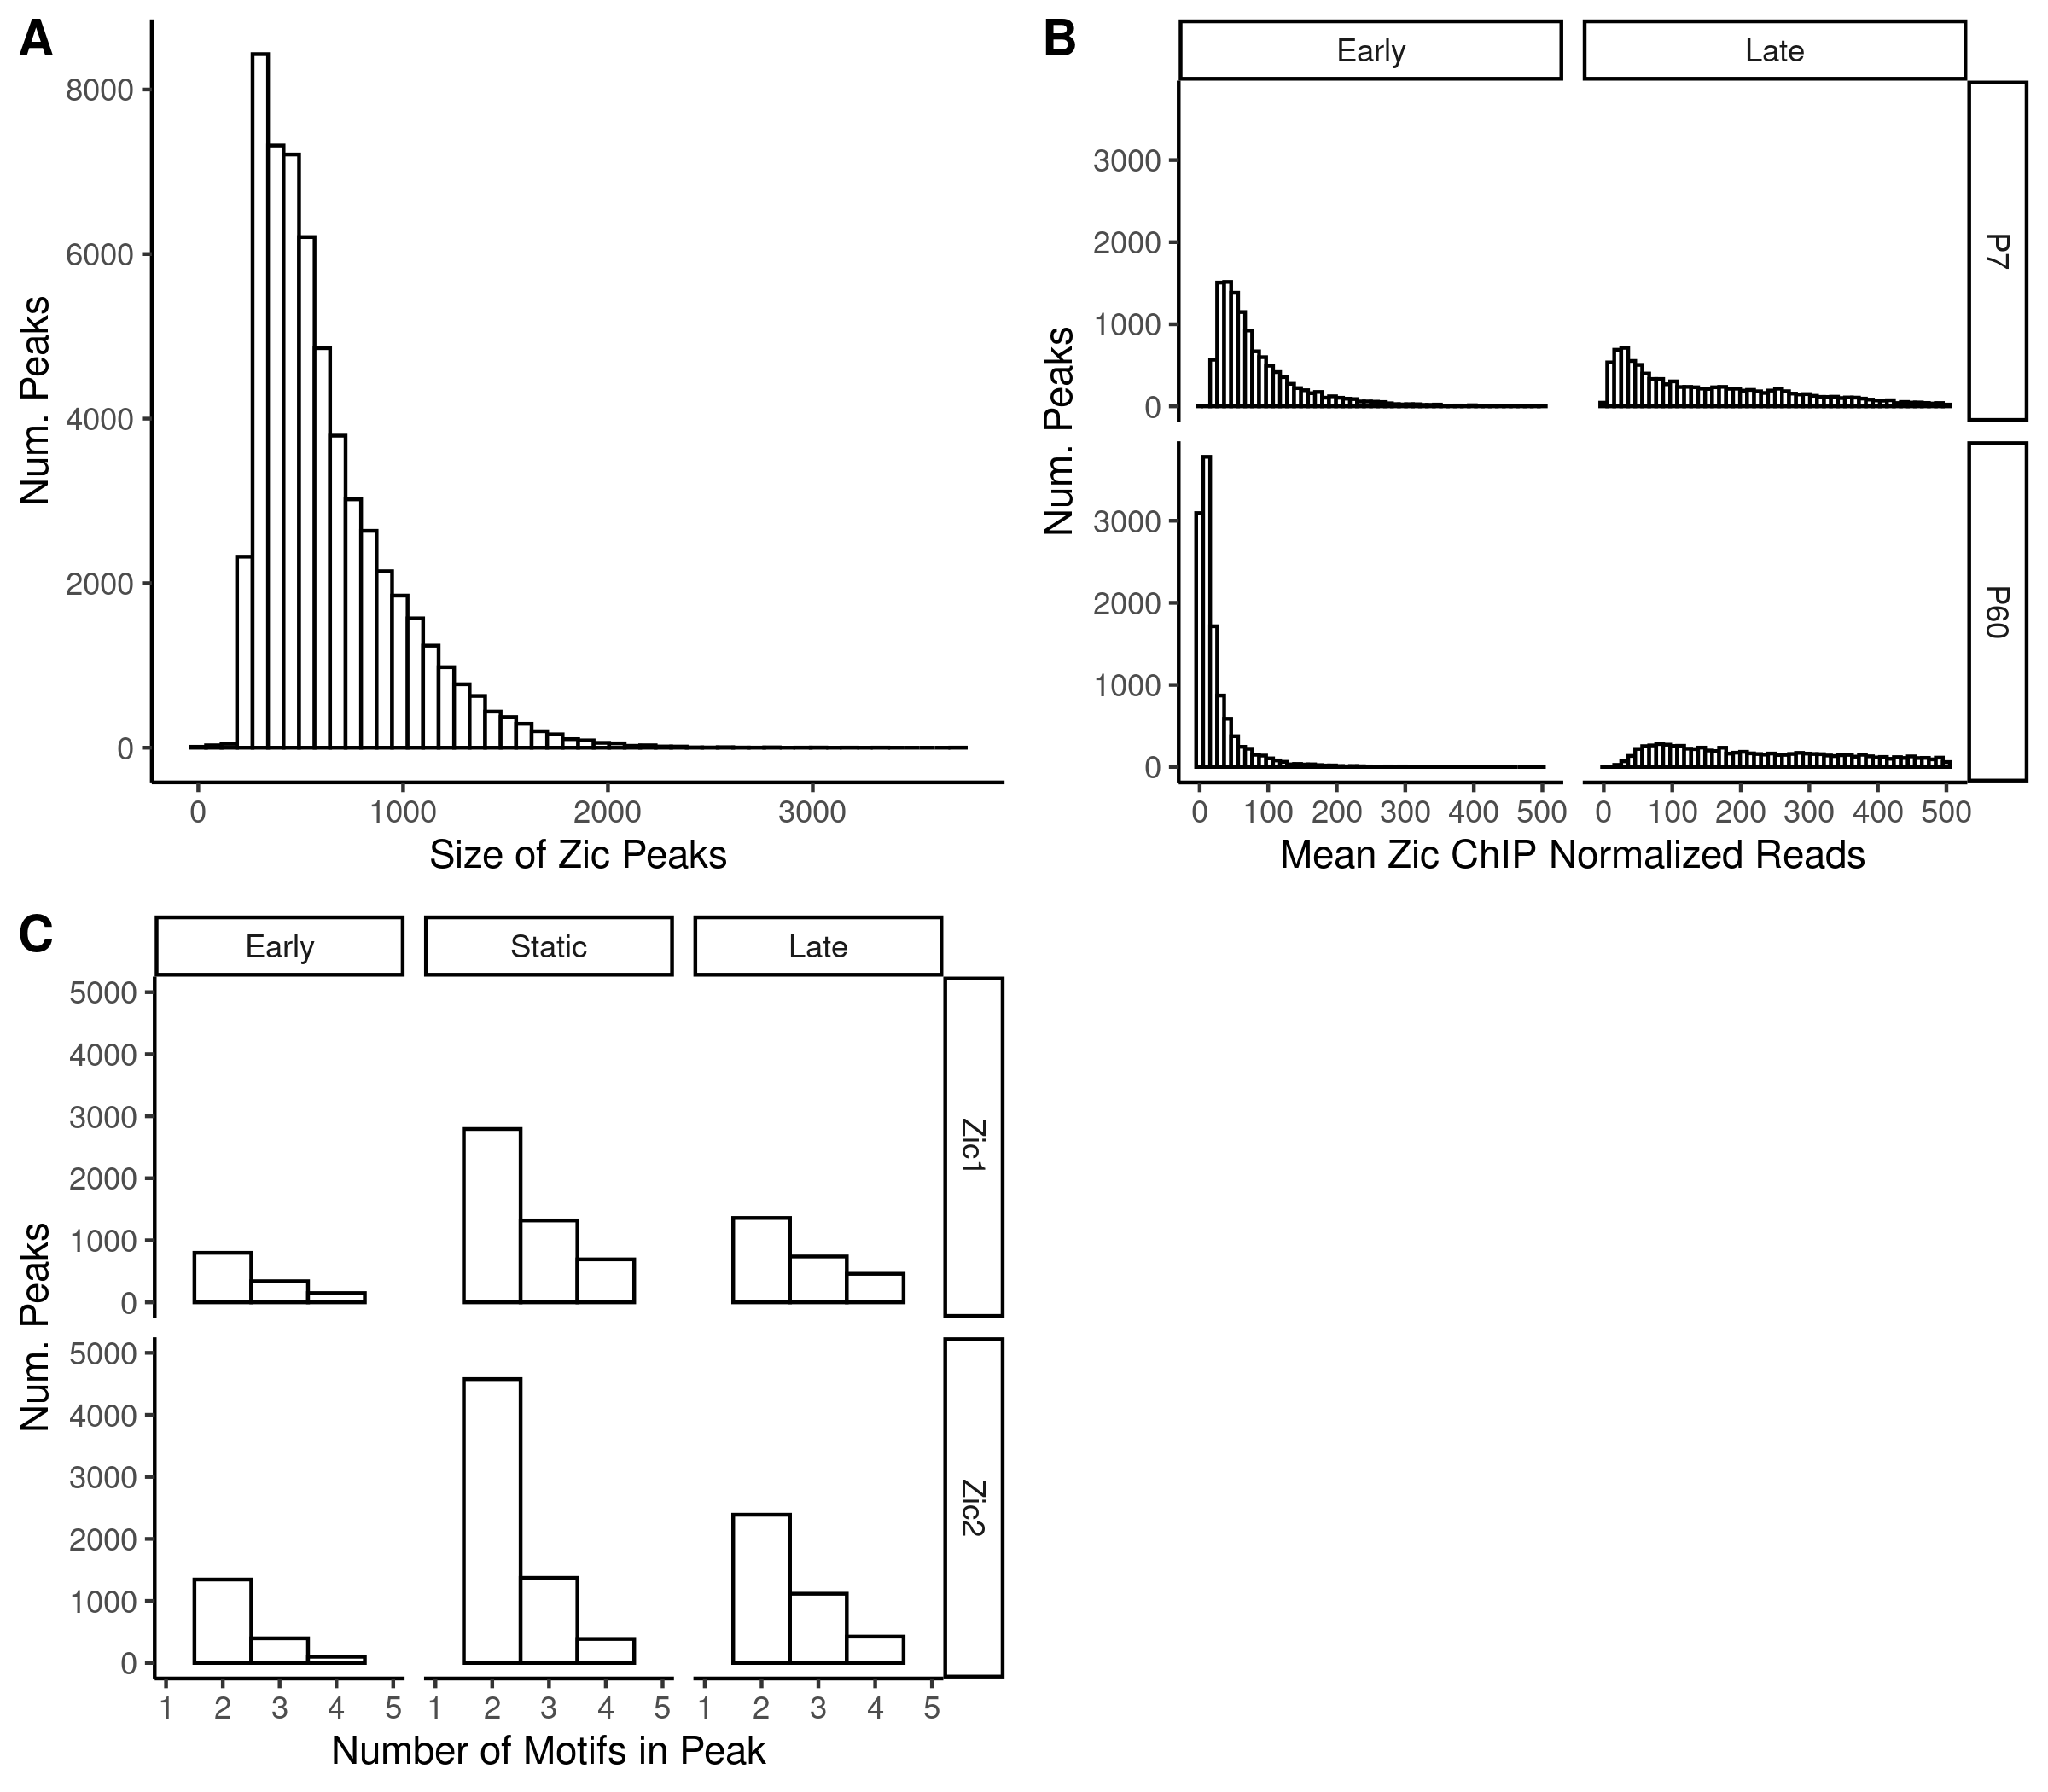
\includegraphics[width=.90\linewidth]{Figures/supp_figure1.png}
\caption{A) Distribution of Zic peak size. Average ChIP signal of peaks at B) P7 and C) P60. D) MA plot of Zic-ChIP peaks P7 v P60. E) Number of peaks whose mean ChIP signal is 0 at P7 or P60}
\label{fig:ZicStats}
\end{figure*}


\begin{figure*}[ht]
\centering
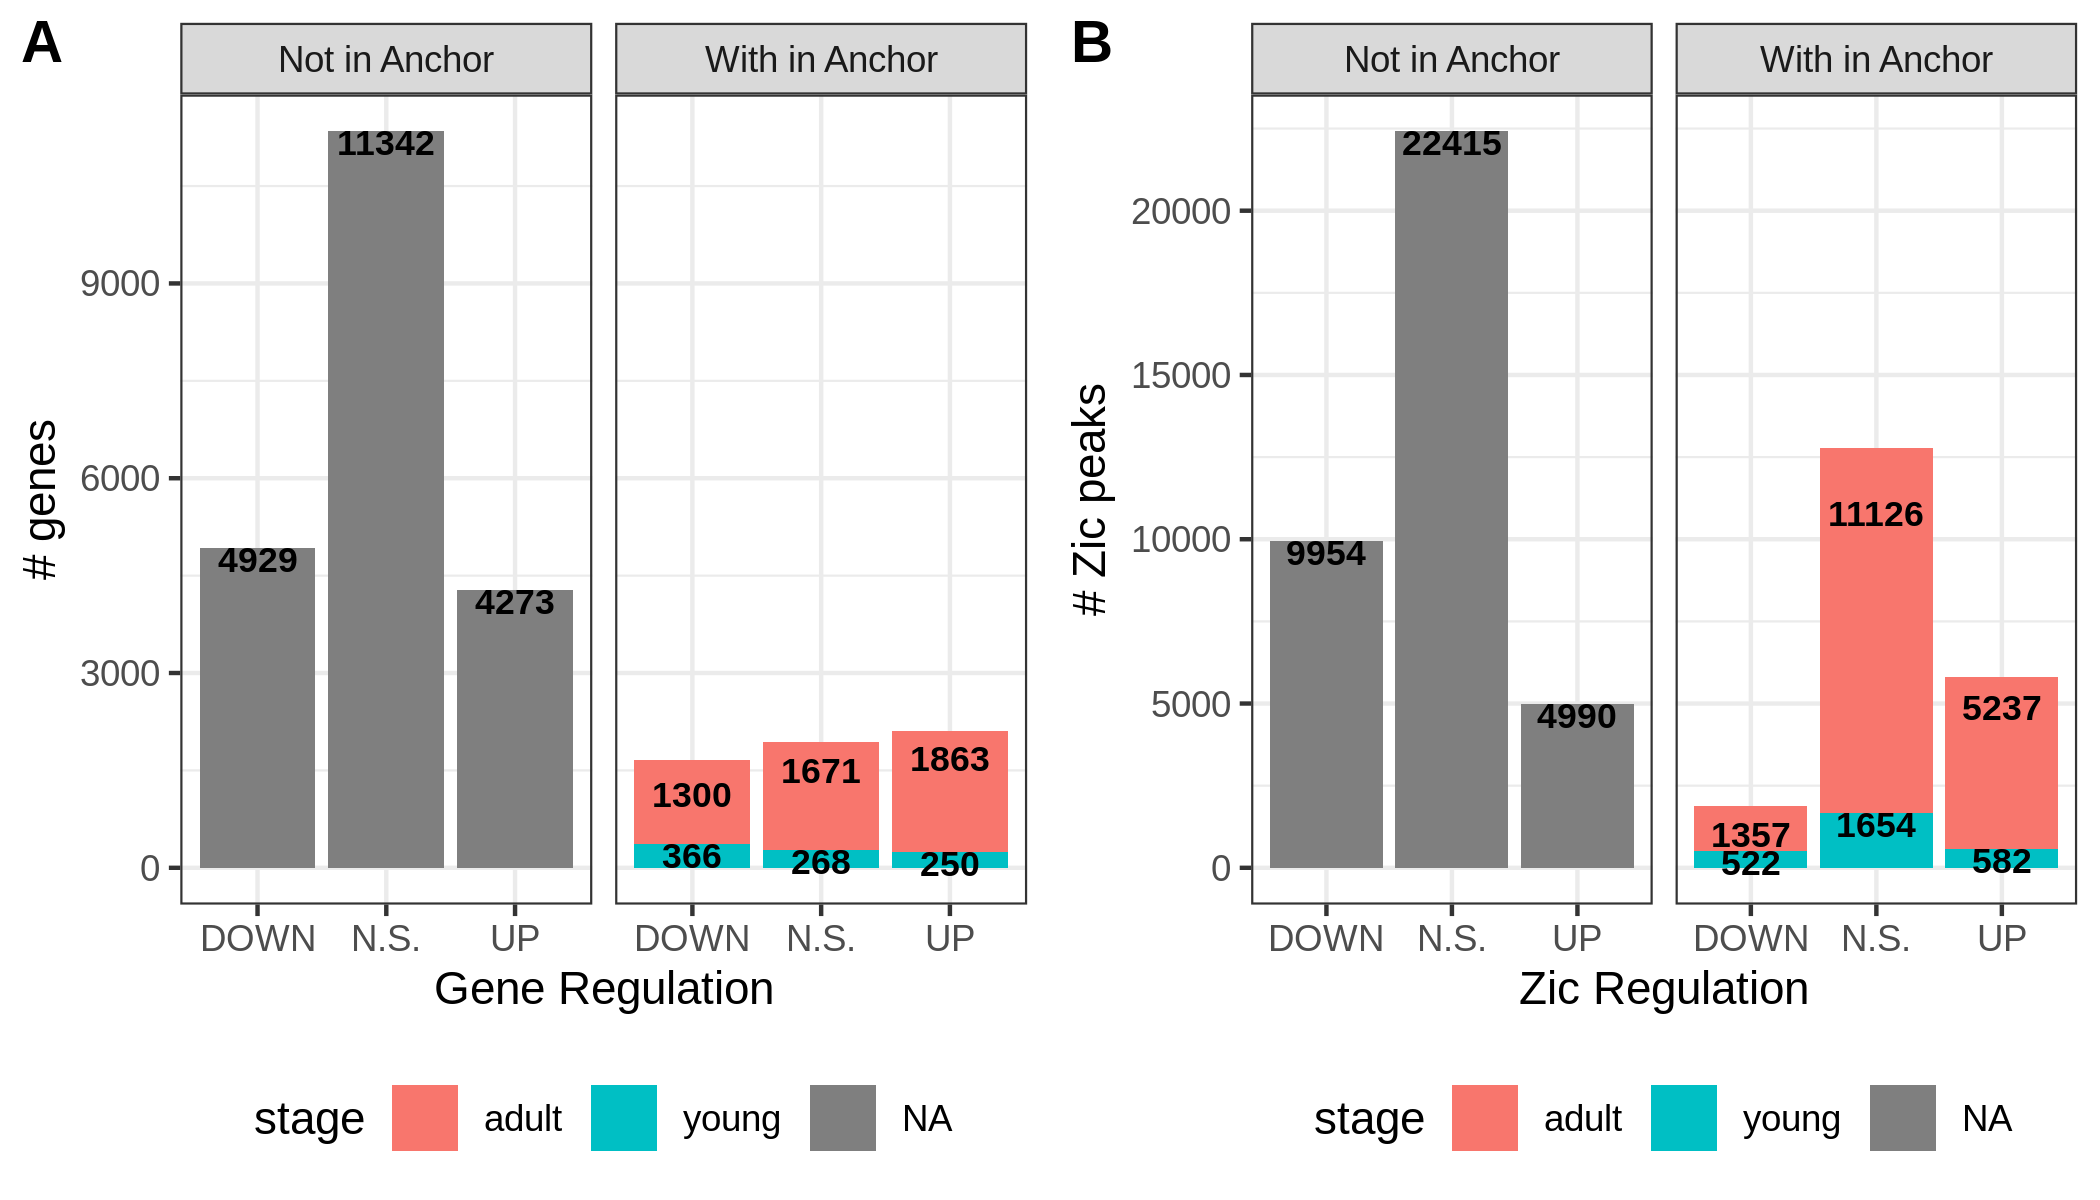
\includegraphics[width=.90\linewidth]{Figures/supp_figure2.png}
\caption{Mapping statistics of A) Nearest gene, B) Zic, C) DNase, and D) H3K27ac peaks in H4Kme3 PLAC-seq derived chromatin loops.}
\label{fig:MappingStats}
\end{figure*}


\begin{figure*}[ht]
\centering
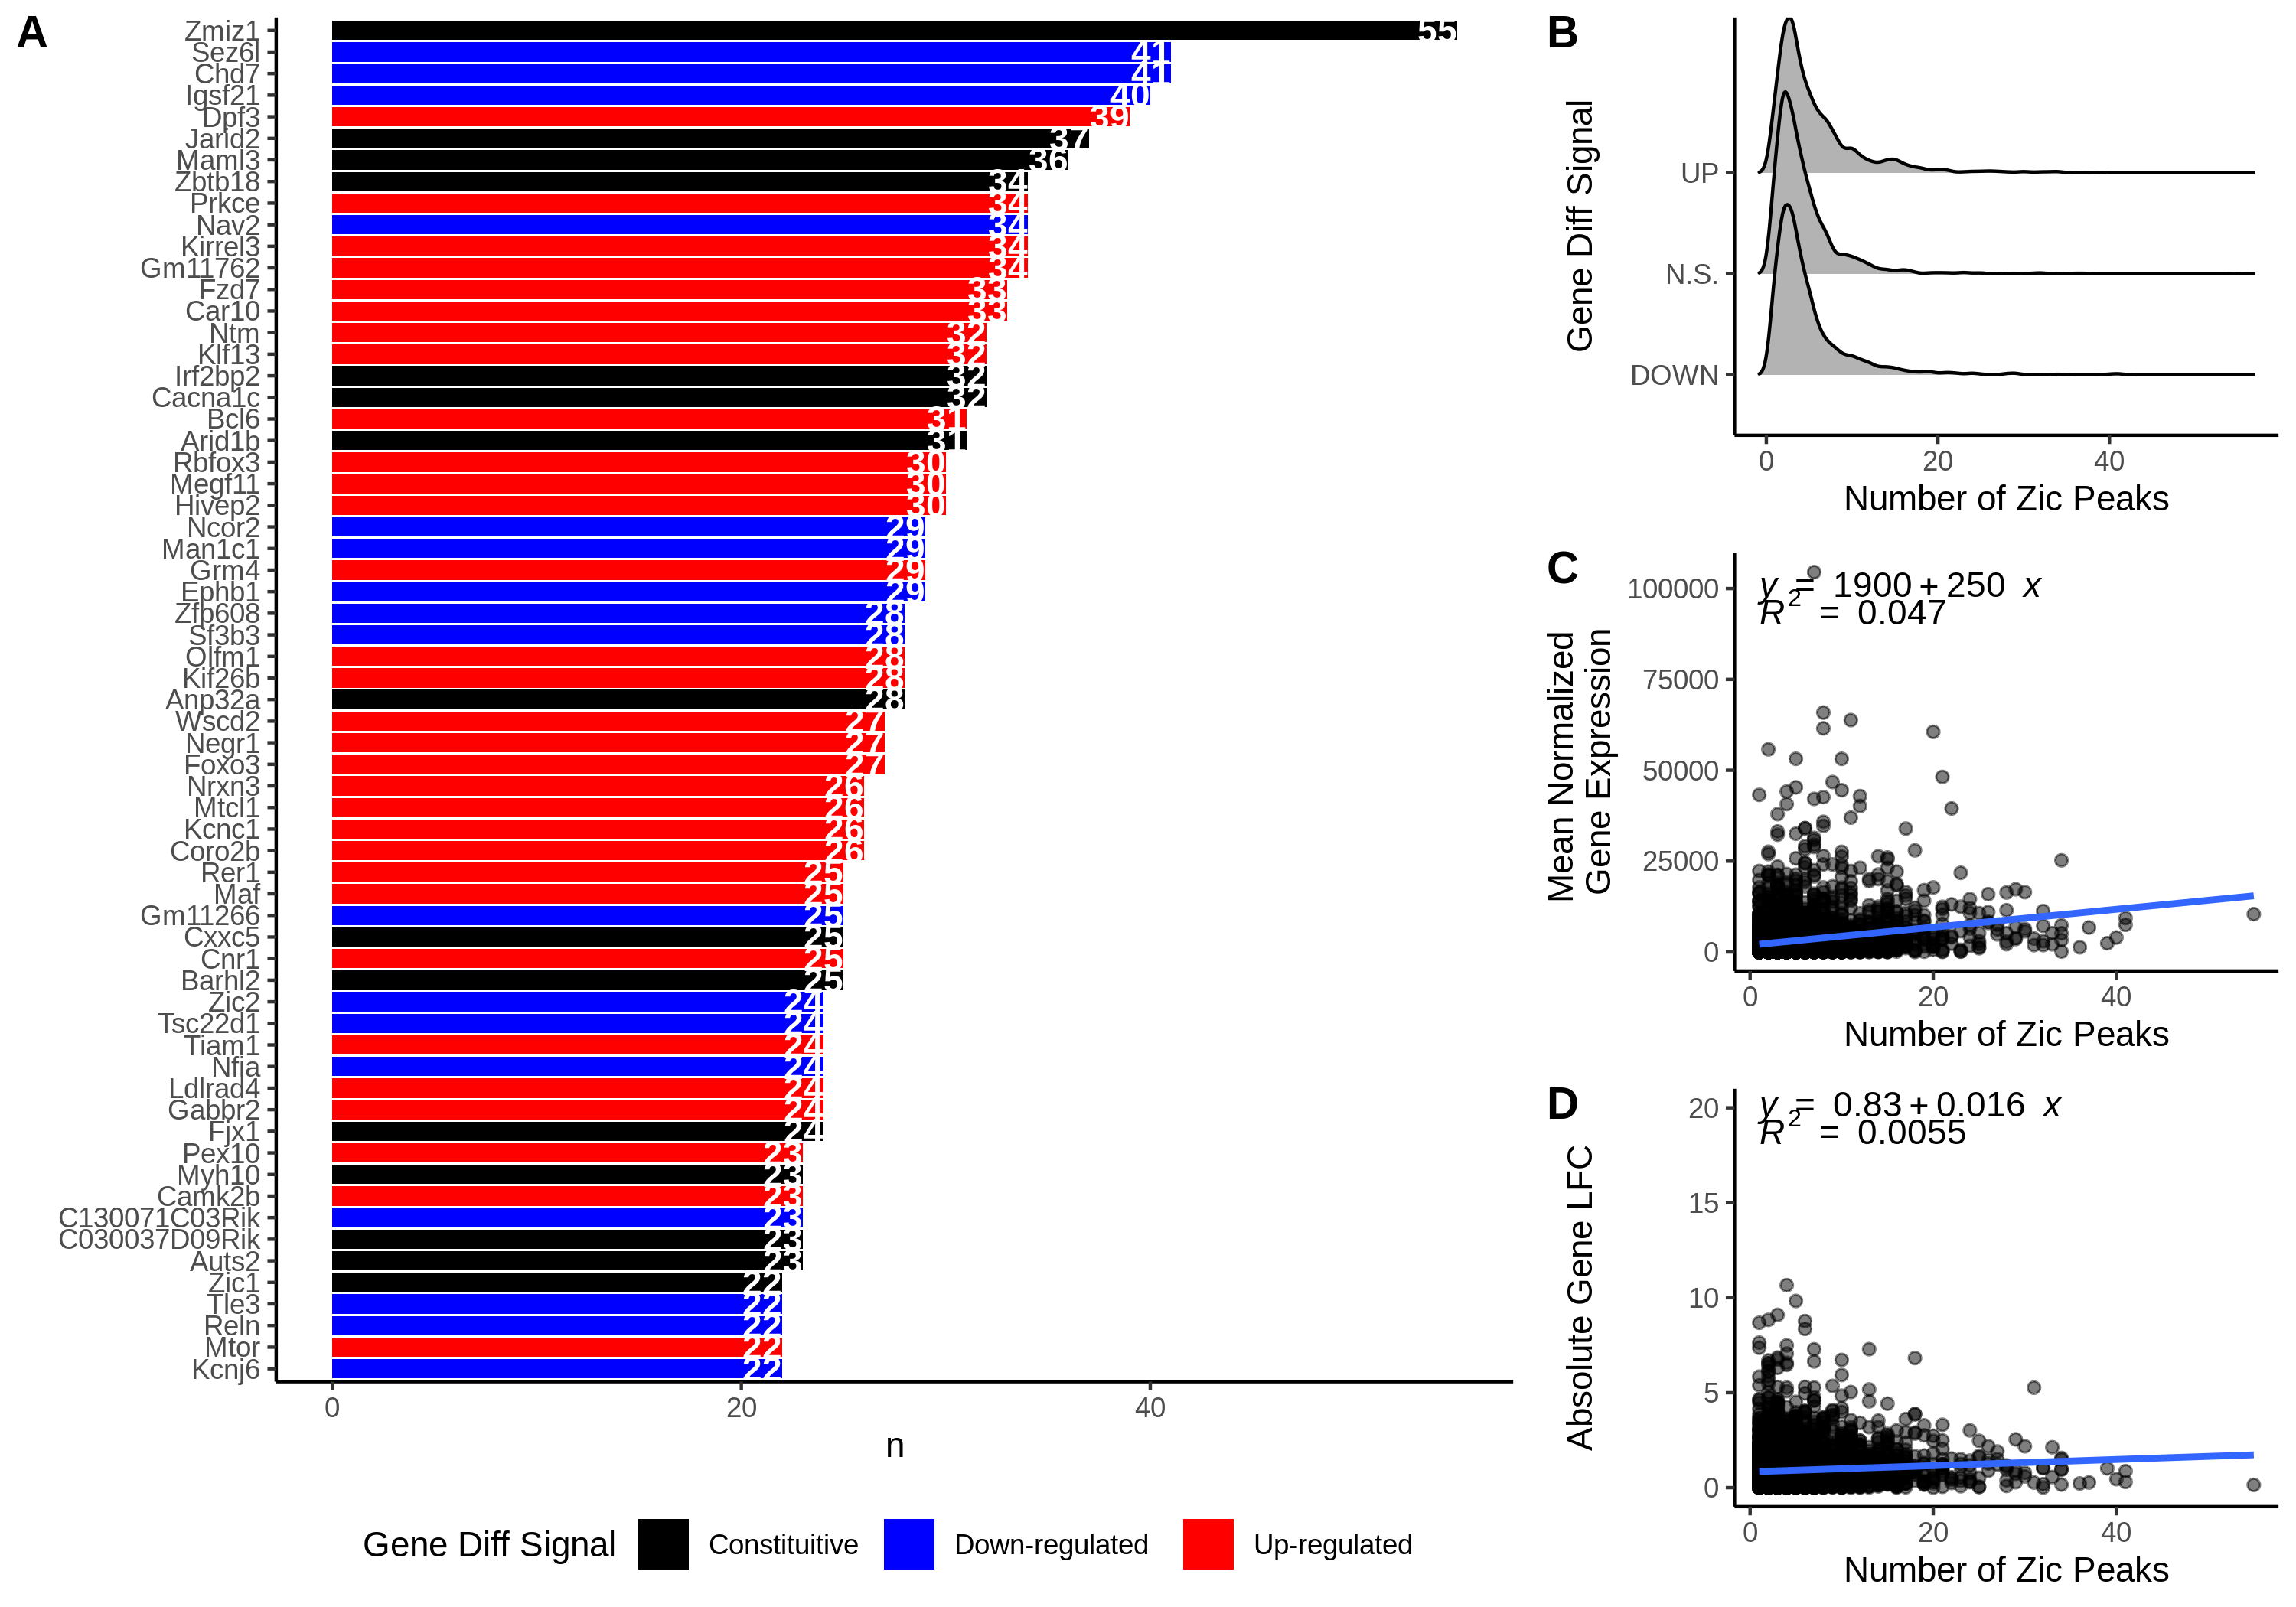
\includegraphics[width=.90\linewidth]{Figures/supp_figure3.png}
\caption{ A) Count of Zic peaks mapped to gene. B) Distribution of number of Zic peaks by gene regulation.  Scatter-plots of C) Mean expression and D) Log2FC of genes against Number of Zic peaks show that there is no correlation between number of Zic peaks and gene degree of gene regulation. }
\label{fig:nPeakstoGenes}
\end{figure*}


\begin{figure*}[ht]
\centering
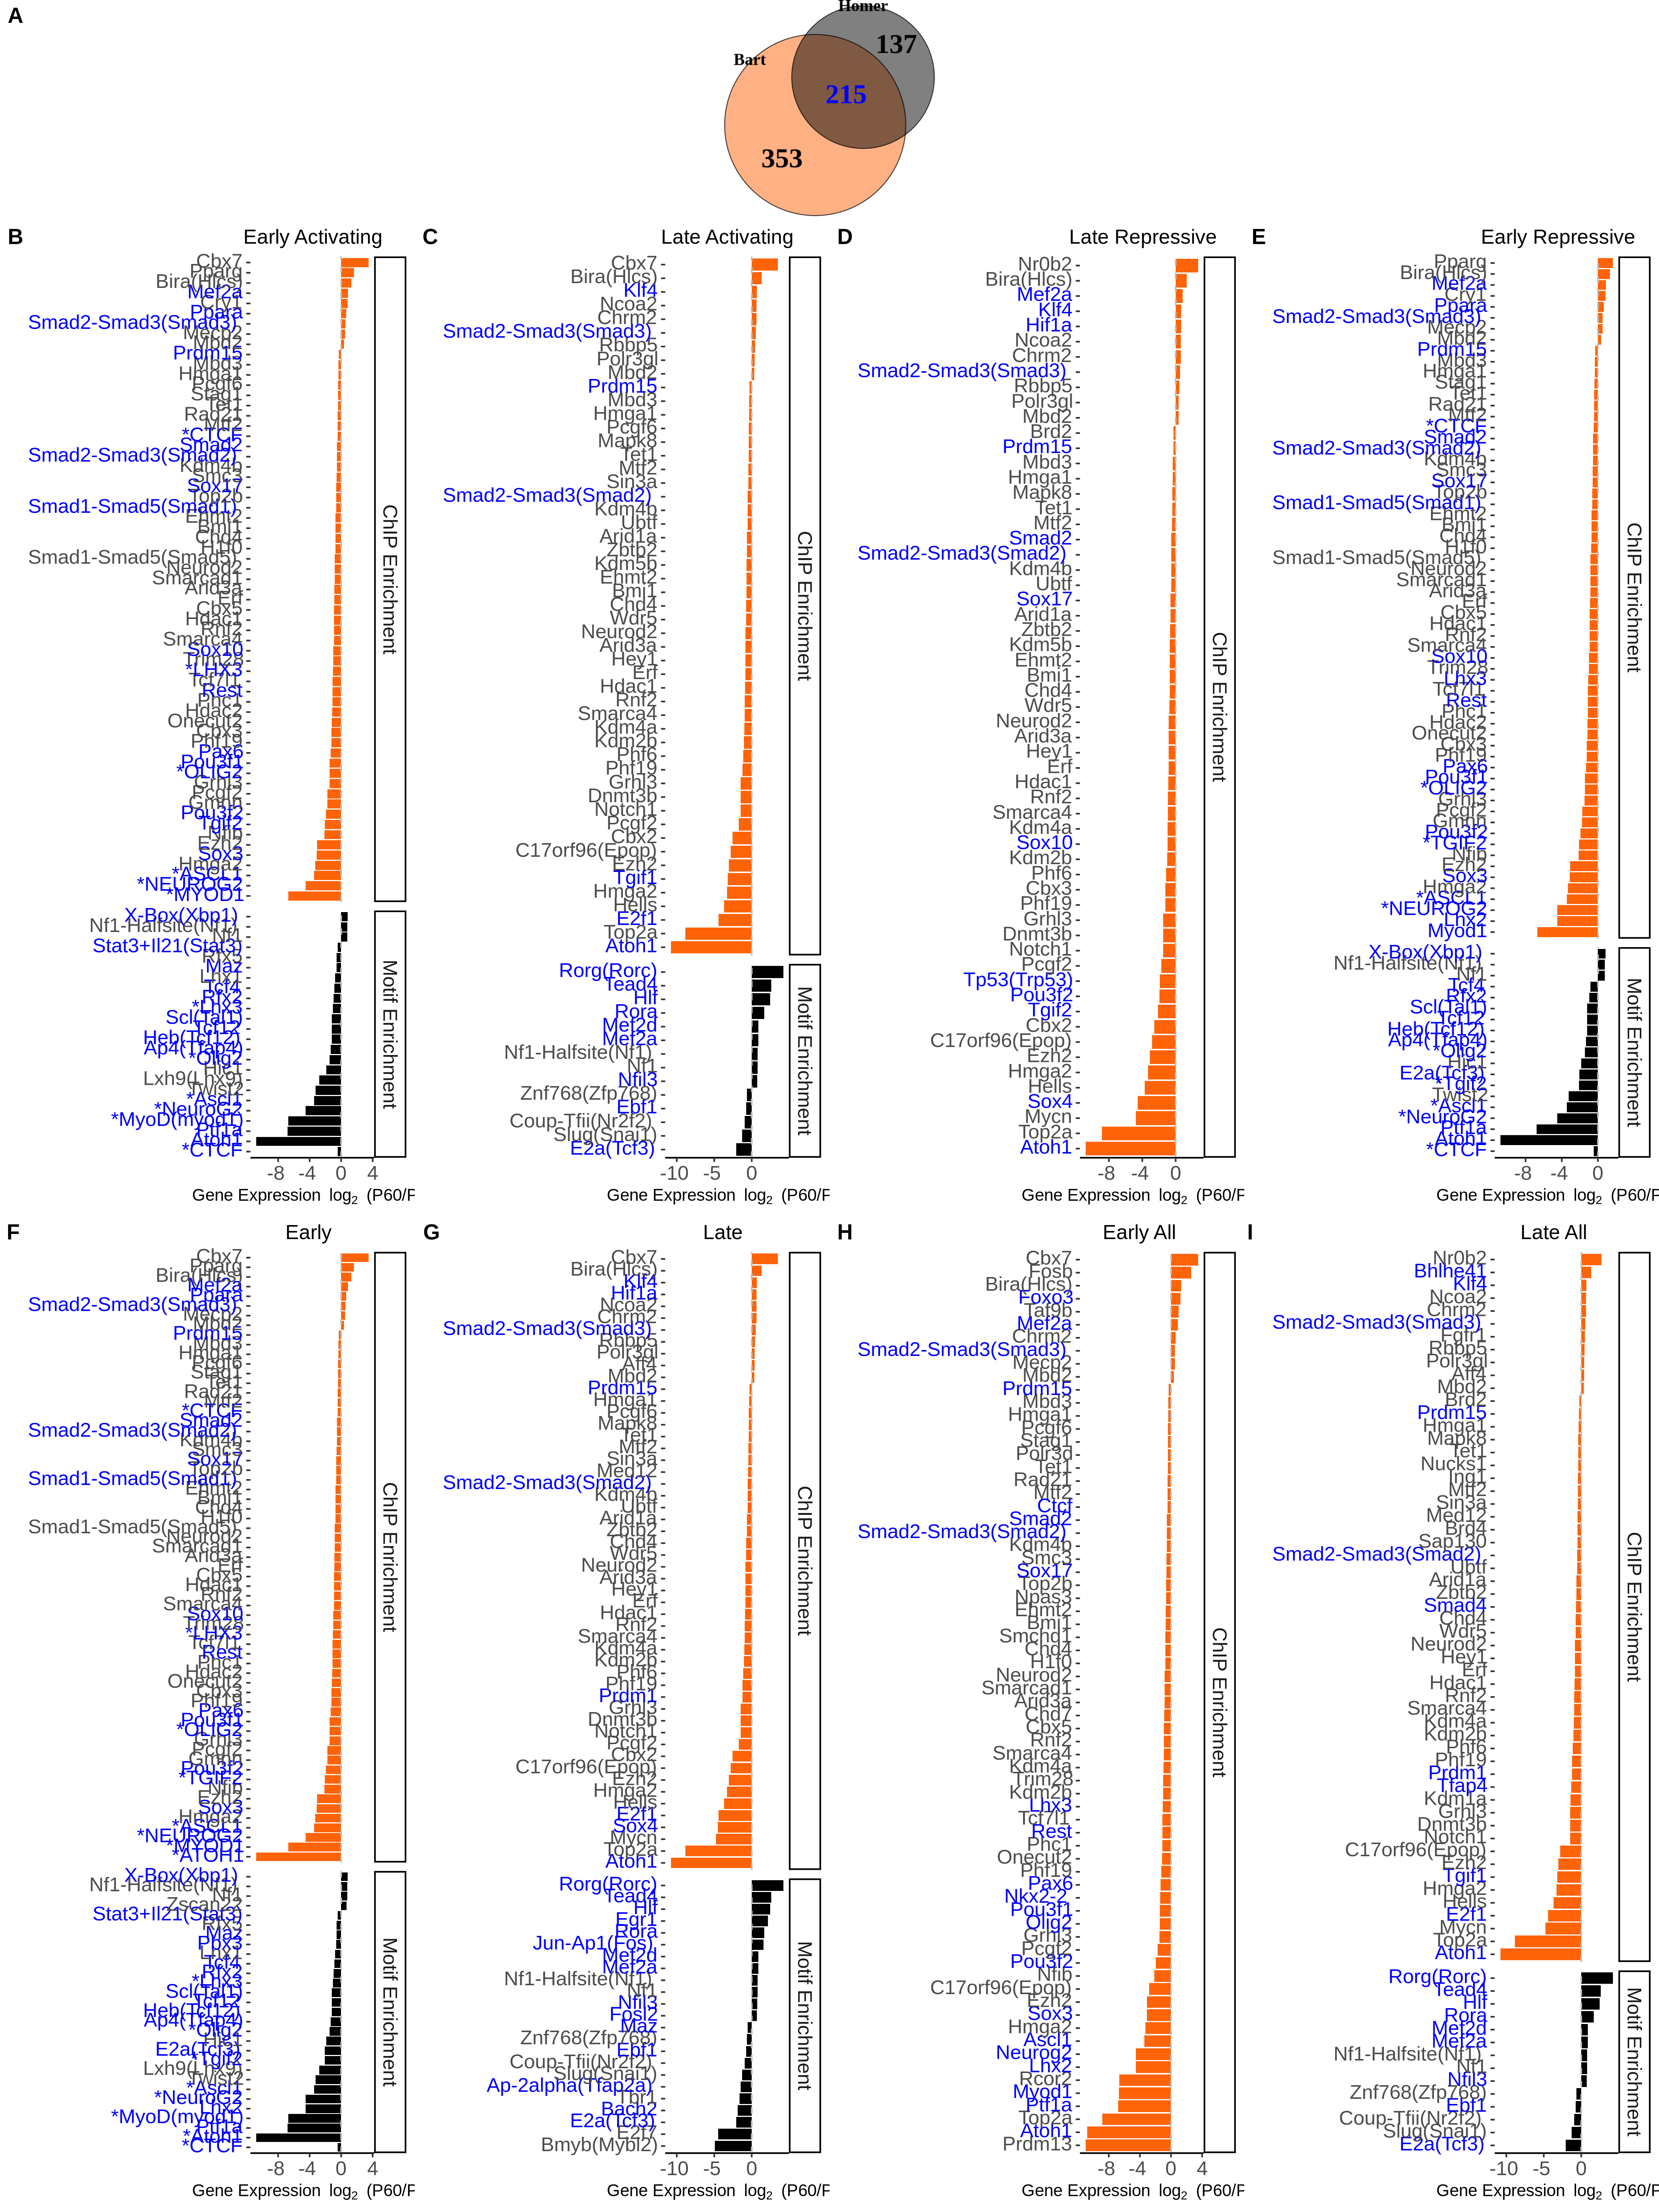
\includegraphics[width=.95\textwidth]{Figures/supp_figure4.png}
\caption{Mouse in-vivo ChIP overlap enrichment (BART) and motif enrichment (HOMER) of Zic ChIP peaks that were separated by mapped gene expression into A) Early Activating, B) Late Activating c) Early Repressive D) Late Repressive. *Denotes predicted TFs that are common between the ChIP overlap enrichment and motif enrichment. }
\label{fig:HomerBart}
\end{figure*}

\begin{figure*}[ht]
\centering
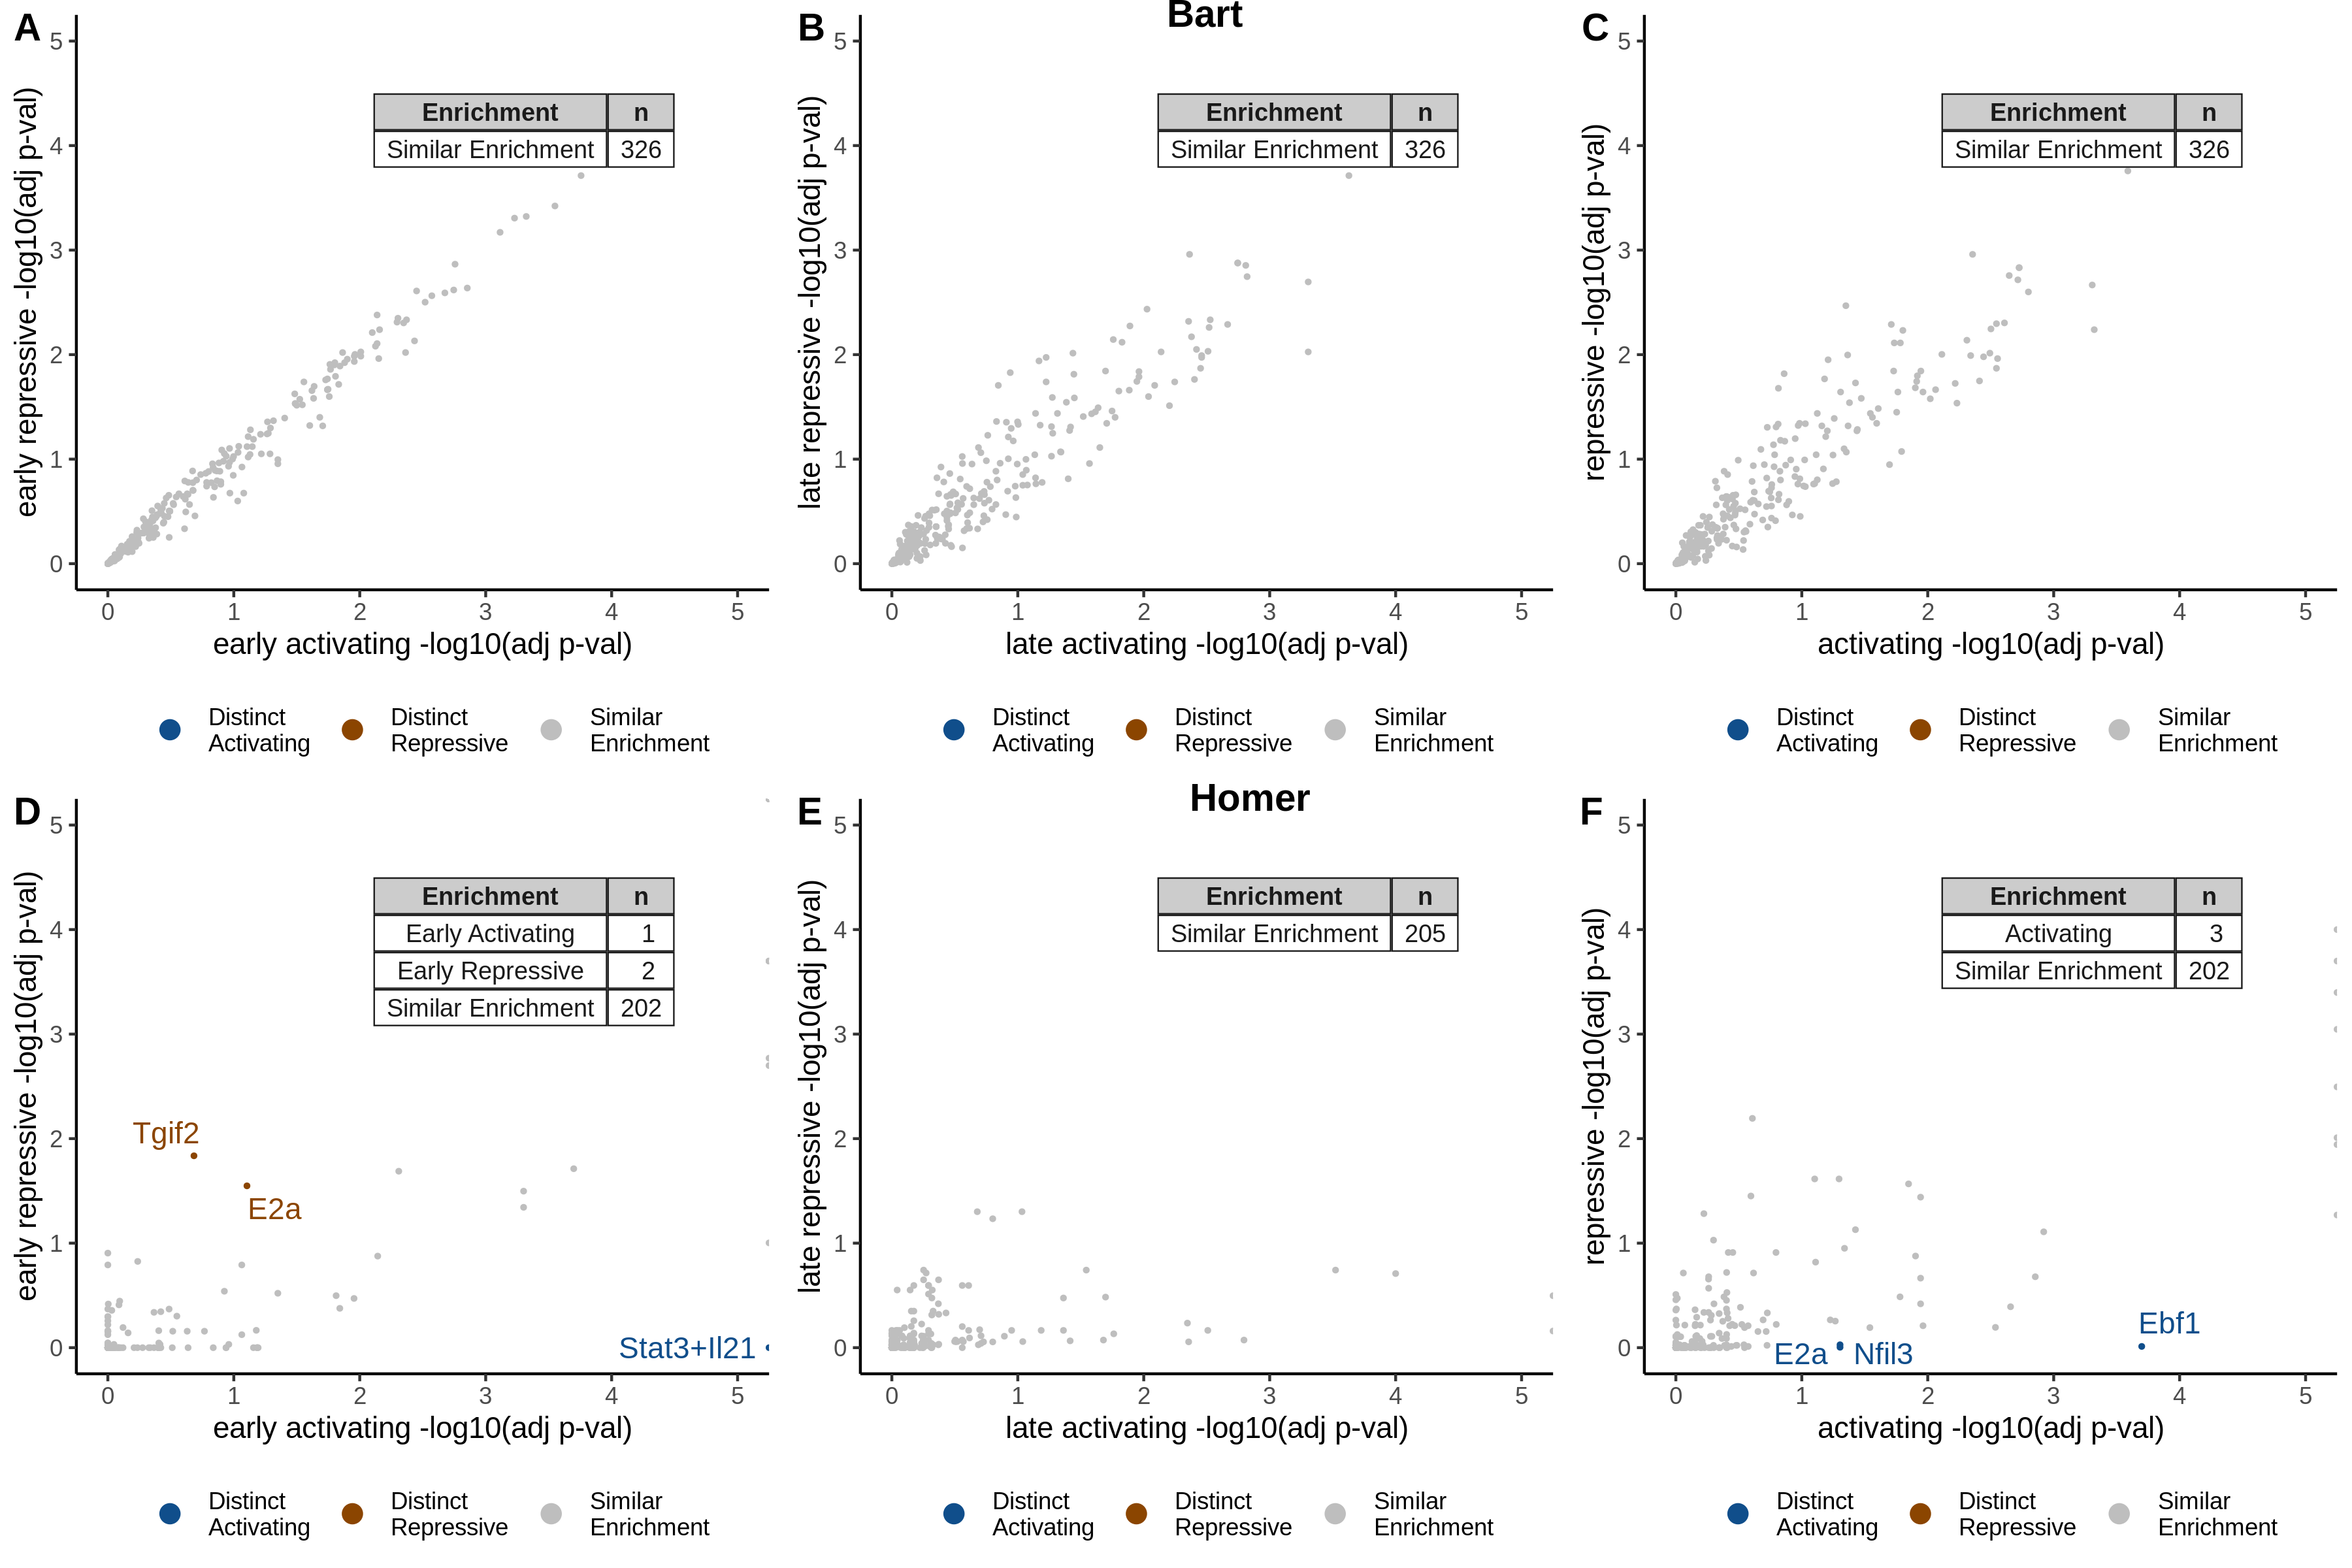
\includegraphics[width=.95\textwidth]{Figures/supp_figure_rrho.png}
\caption{Zic peaks were classified into activating or repressive sets based on the map gene and the regulation of the Zic peaks. When calculating the distinctly enriched TFs between the A,D) early activating and repressive, B,E) late activating and repressive, C,F) all activating v repressive}
\label{fig:ActvRep}
\end{figure*}

\begin{figure*}[ht]
\centering
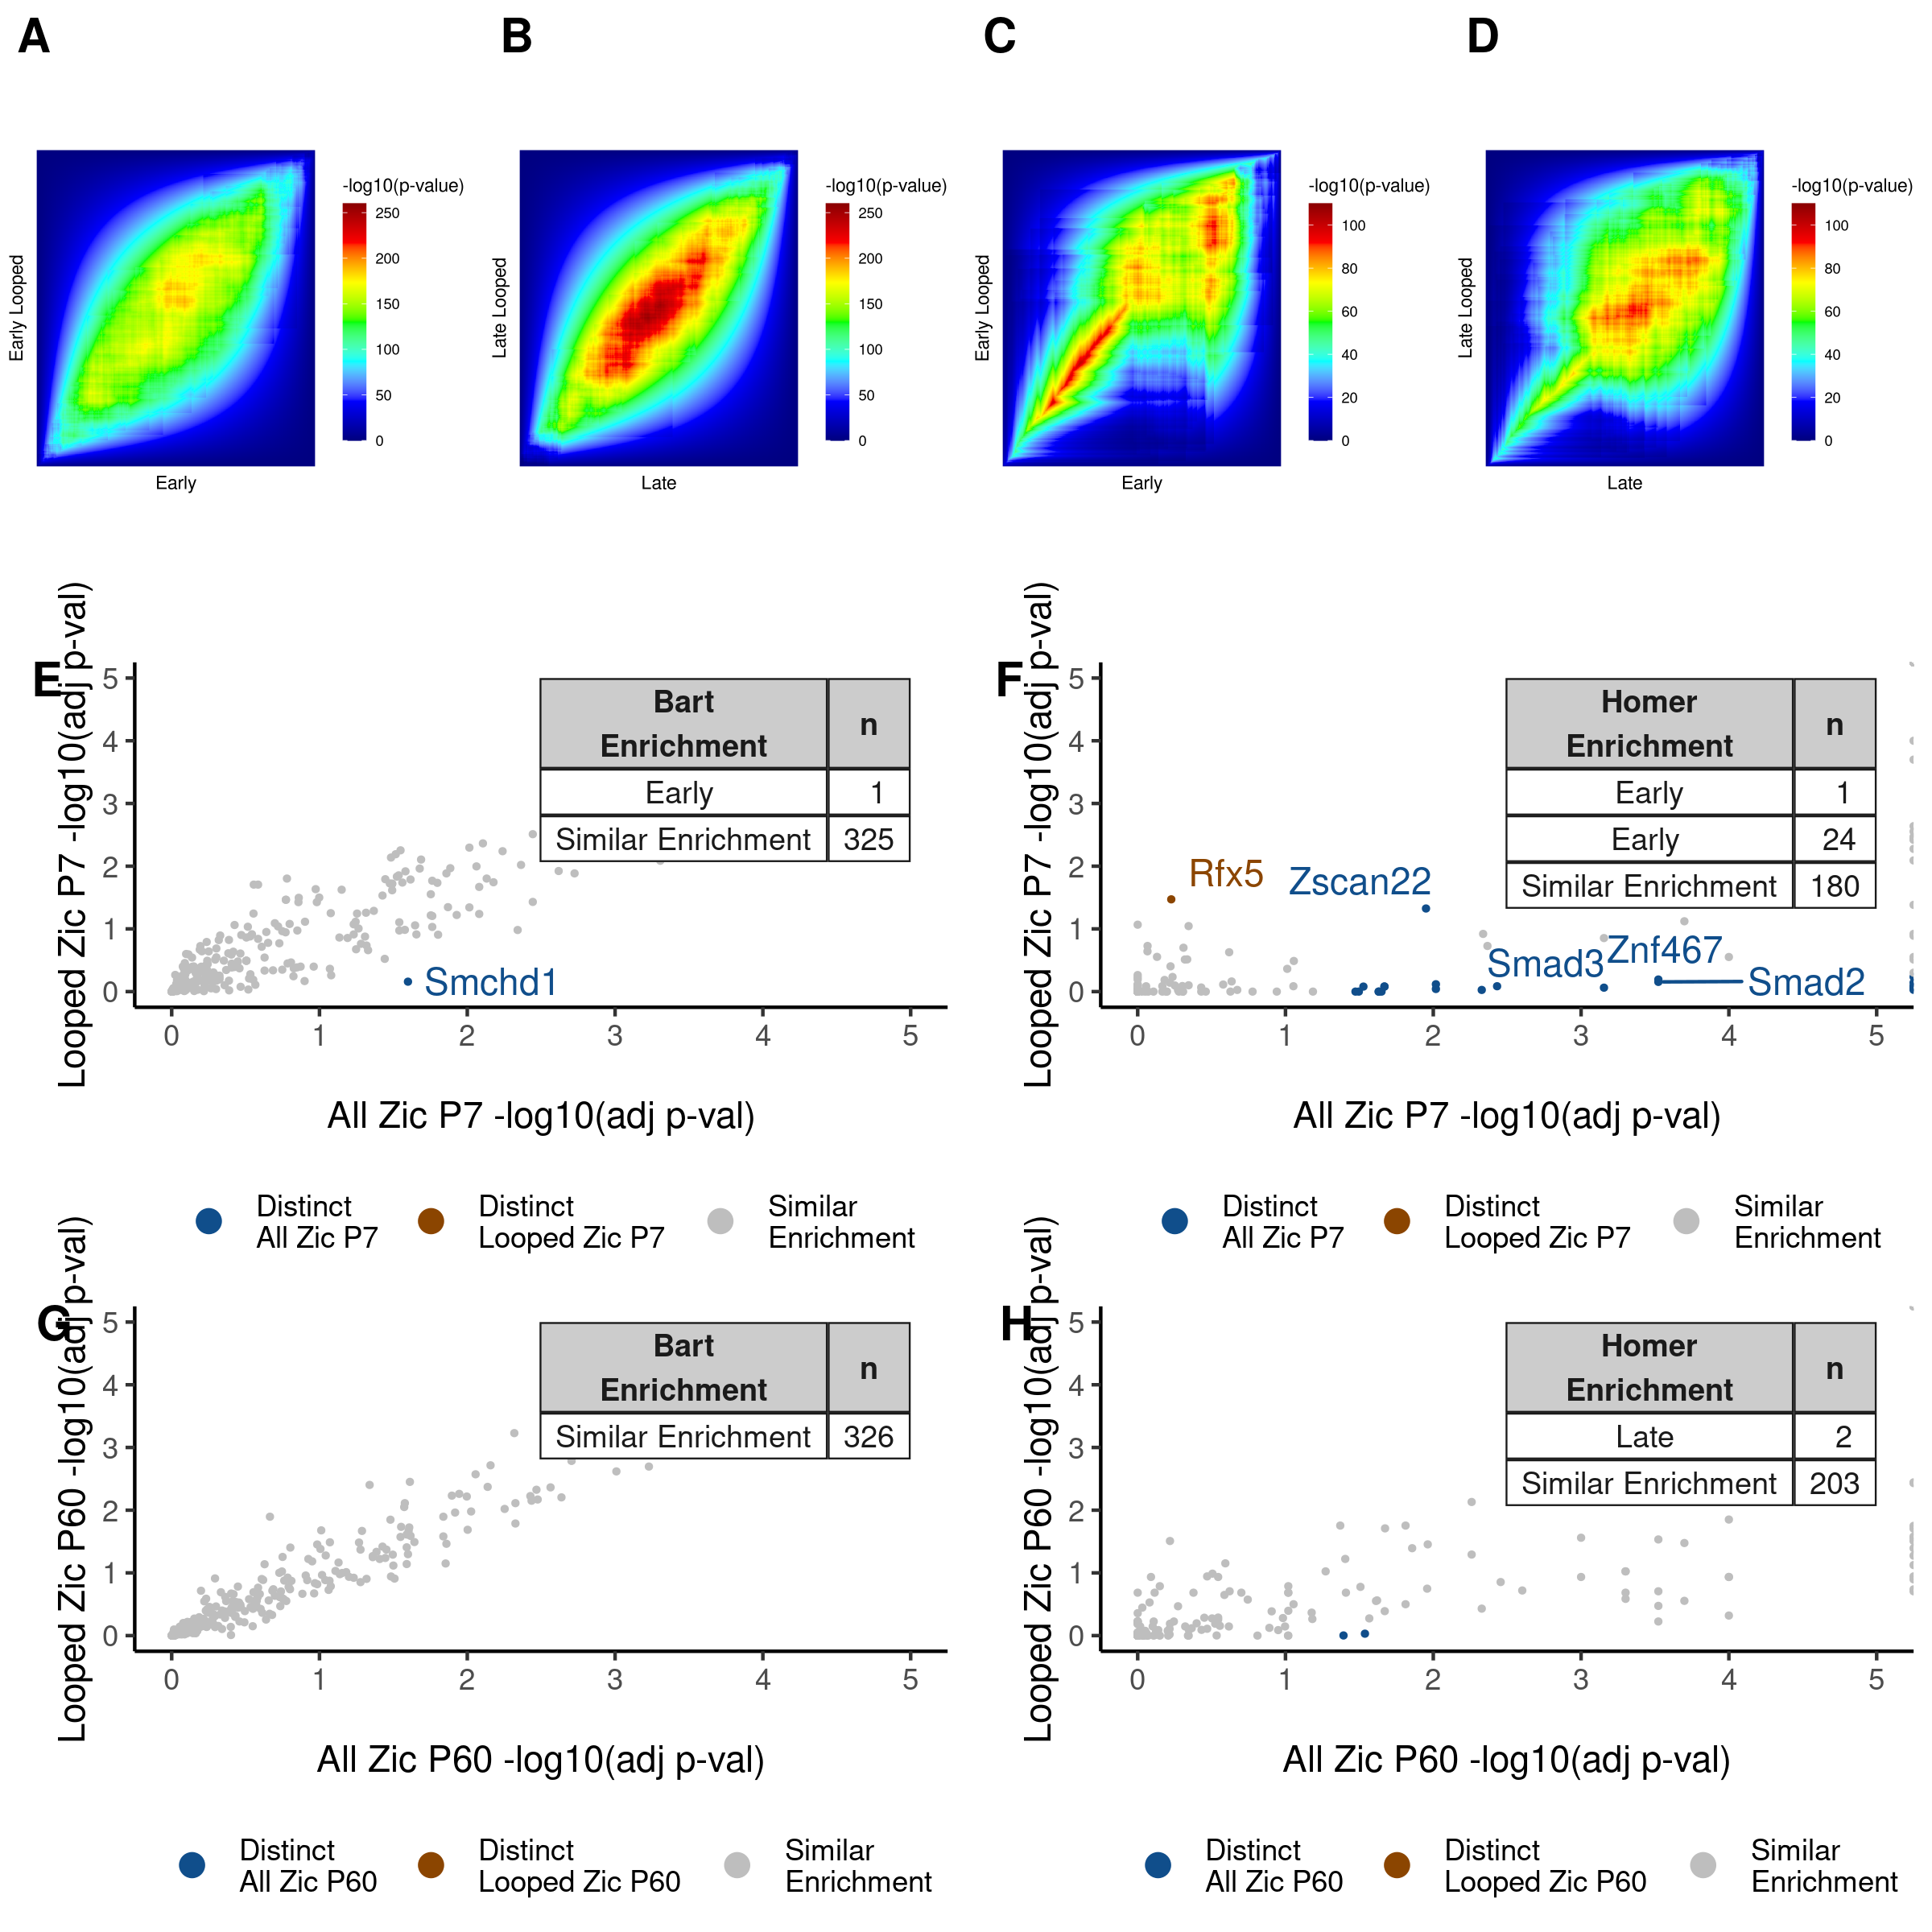
\includegraphics[width=.95\textwidth]{Figures/supp_figure_rrho_allvlooped.png}
\caption{Distinct TFs between the all Zic1/2 ChIP sites and the ones within anchors}
\label{fig:loopved_all}
\end{figure*}


\begin{figure*}[ht]
\centering
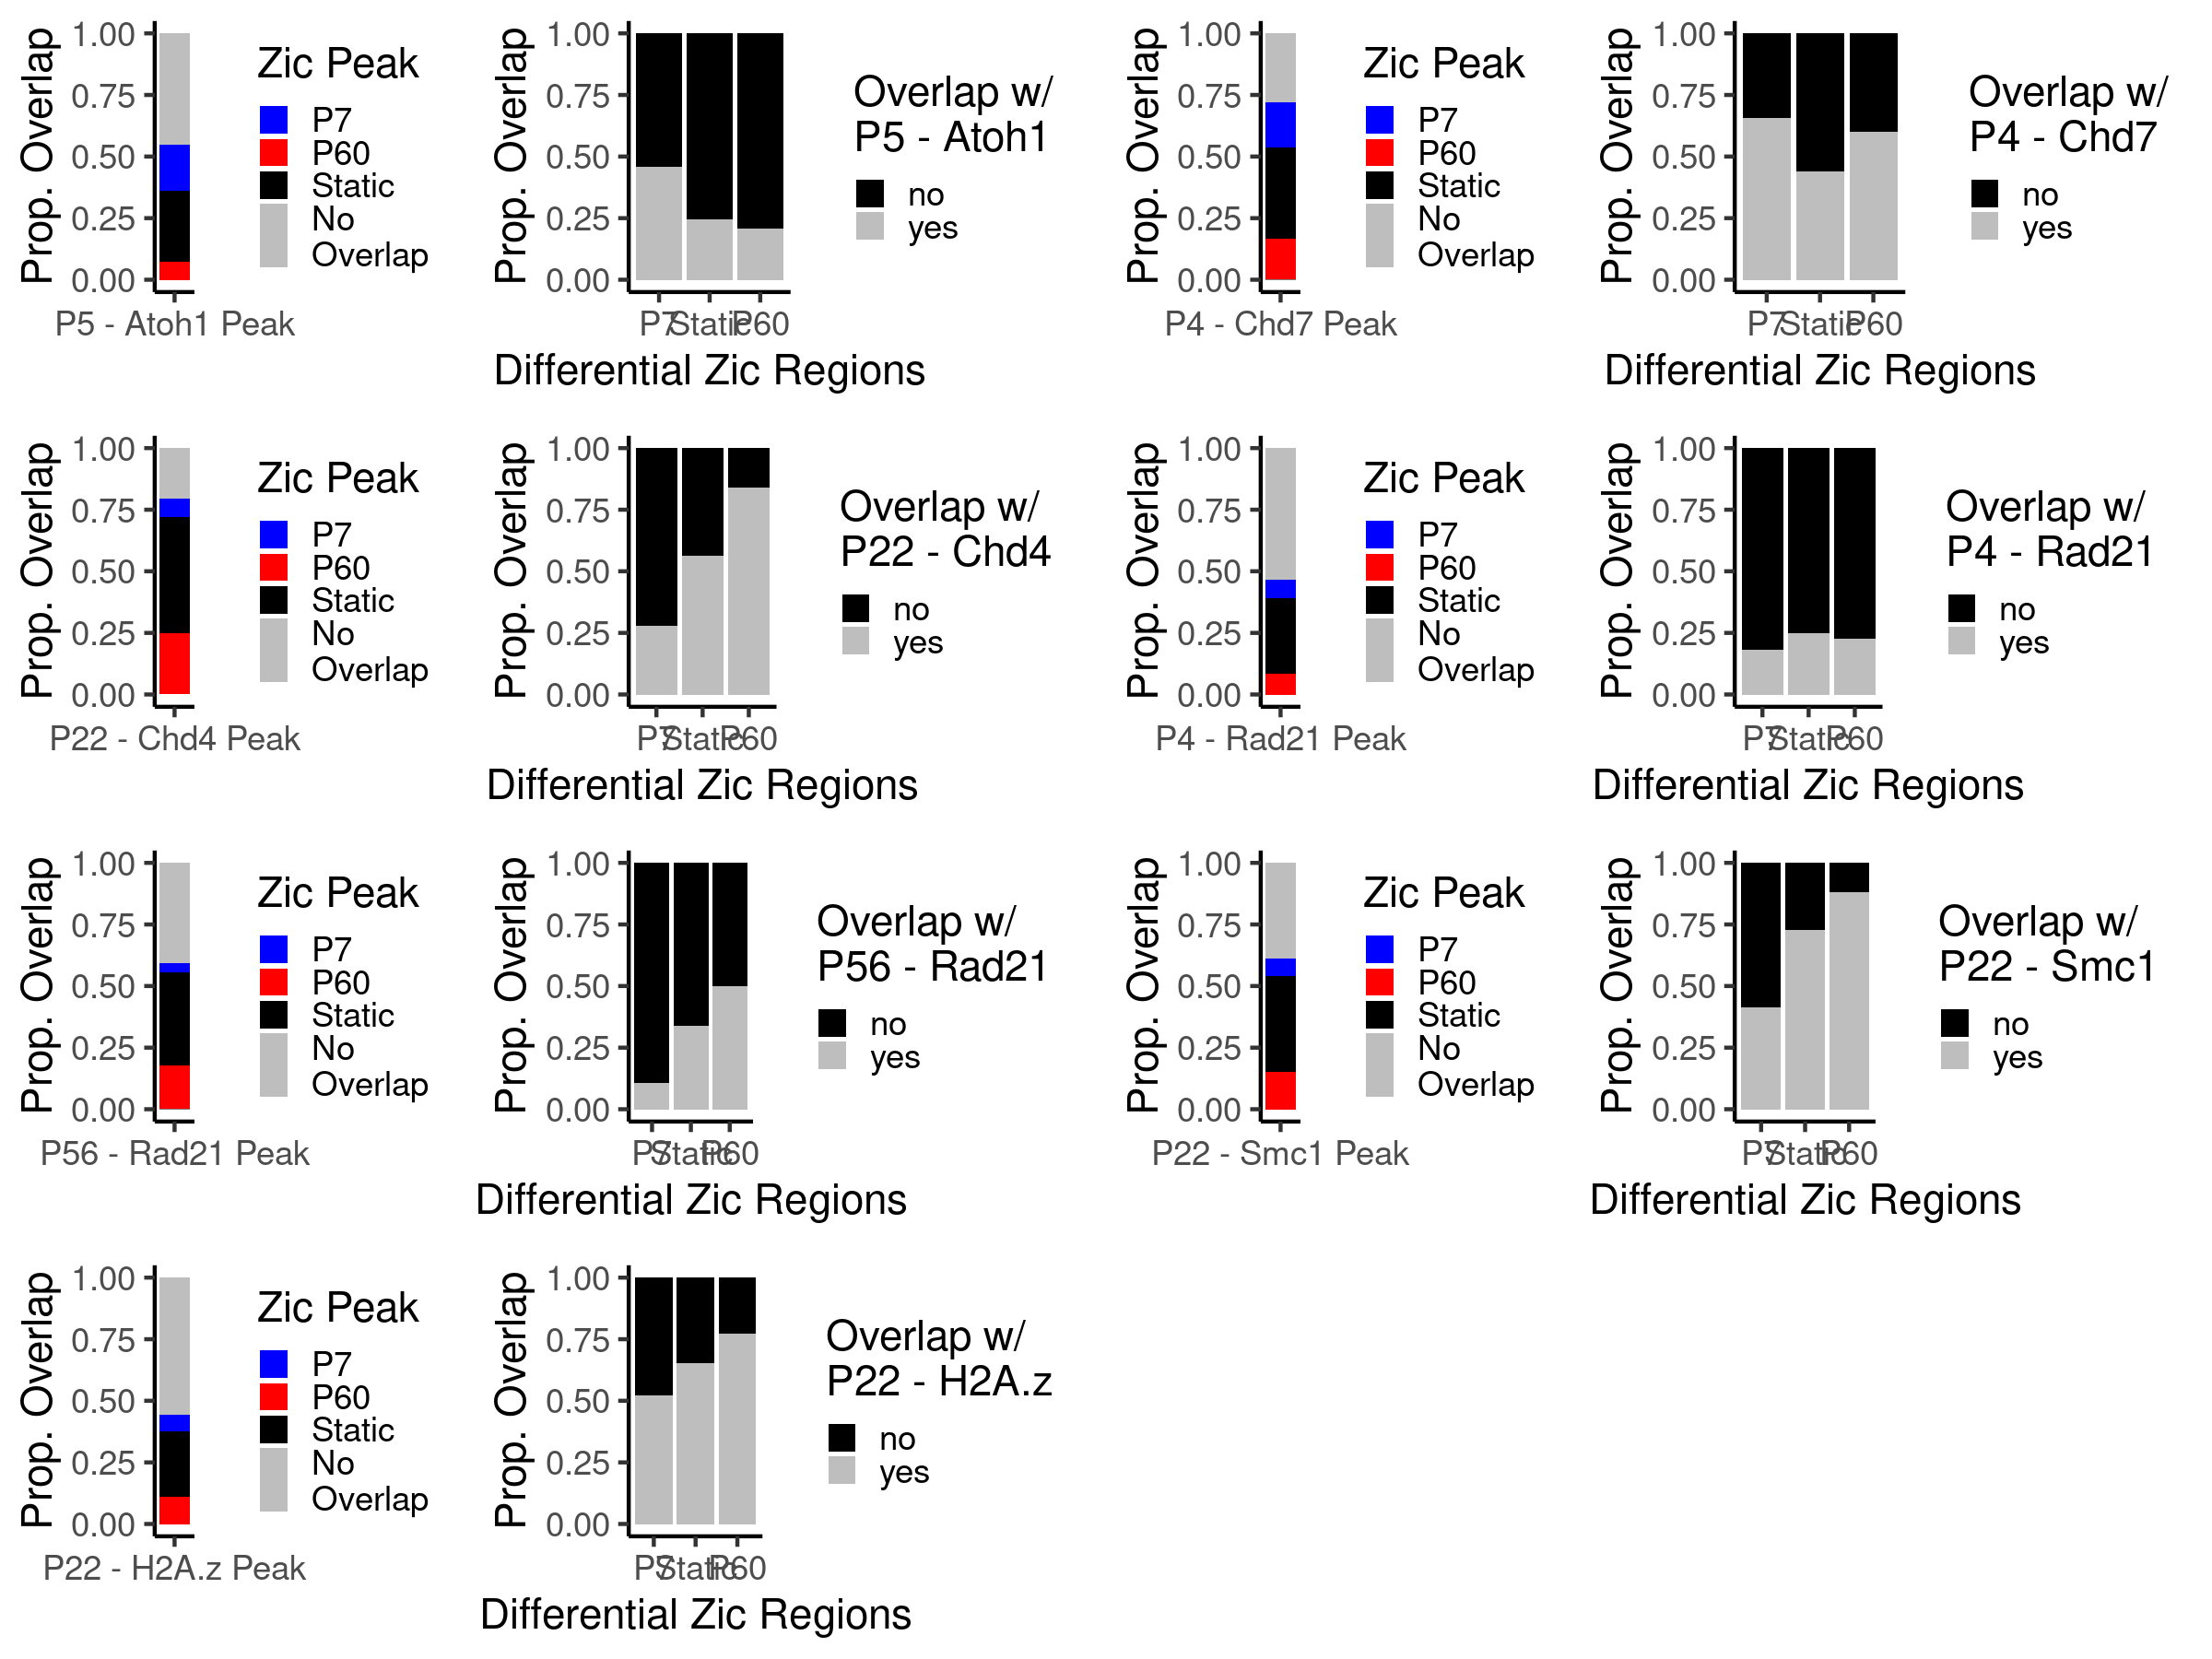
\includegraphics[width=.95\textwidth]{Figures/supp_figure_chip_overlap.png }
\caption{Percent overlap of ChIP-seq datasets in mouse cerebellum and Zic1/2 ChIP-seq}
\label{fig:chip_overlap}
\end{figure*}




\end{document}